\pdfbookmark{Общая характеристика работы}{characteristic}             % Закладка pdf
\section*{Общая характеристика работы}

\newcommand{\actuality}{\pdfbookmark[1]{Актуальность}{actuality}\underline{\textbf{\actualityTXT}}}
\newcommand{\progress}{\pdfbookmark[1]{Разработанность темы}{progress}\underline{\textbf{\progressTXT}}}
\newcommand{\aim}{\pdfbookmark[1]{Цели}{aim}\underline{{\textbf\aimTXT}}}
\newcommand{\tasks}{\pdfbookmark[1]{Задачи}{tasks}\underline{\textbf{\tasksTXT}}}
\newcommand{\aimtasks}{\pdfbookmark[1]{Цели и задачи}{aimtasks}\aimtasksTXT}
\newcommand{\novelty}{\pdfbookmark[1]{Научная новизна}{novelty}\underline{\textbf{\noveltyTXT}}}
\newcommand{\influence}{\pdfbookmark[1]{Практическая значимость}{influence}\underline{\textbf{\influenceTXT}}}
\newcommand{\methods}{\pdfbookmark[1]{Методология и методы исследования}{methods}\underline{\textbf{\methodsTXT}}}
\newcommand{\defpositions}{\pdfbookmark[1]{Положения, выносимые на защиту}{defpositions}\underline{\textbf{\defpositionsTXT}}}
\newcommand{\reliability}{\pdfbookmark[1]{Достоверность}{reliability}\underline{\textbf{\reliabilityTXT}}}
\newcommand{\probation}{\pdfbookmark[1]{Апробация}{probation}\underline{\textbf{\probationTXT}}}
\newcommand{\contribution}{\pdfbookmark[1]{Личный вклад}{contribution}\underline{\textbf{\contributionTXT}}}
\newcommand{\publications}{\pdfbookmark[1]{Публикации}{publications}\underline{\textbf{\publicationsTXT}}}


{\actuality}
\ifnumequal{\value{myspec}}{0}{
    Здесь могла бы быть актуальность для 05.13.18
}{
В настоящее время разработка и анализ эффективных систем радиосвязи имеет большое значение для народного хозяйства. Одной из актуальных задач в этой области является задача оптимизации направленности фазированных антенных решеток (ФАР), представляющих собой антенные системы, распределение фаз и амплитуд на элементах которых позволяет получать направленное излучение.
%Интенсивность излучения каждого отдельно взятого излучателя такой системы зависит от геометрии самого излучателя и радиочастоты сигнала, поданного на его вход. Характеристика интенсивности излучения антенны в пространстве называется диаграммой направленности.
Будучи собранными в антенную систему,
%и разведенными в пространстве,
излучатели формируют диаграмму направленности, которая зависит от их расположения и конструкции, а также выбора фаз и амплитуд сигналов, подаваемых на вход излучателей. Возможность формирования направленного излучения позволяет достичь увеличения дальности радиосвязи или уменьшить  затраты ресурсов (энергии, площади, занимаемой антеннами, стоимости оборудования и др.).
%Это связано с тем, что часть излучения итерферирует с собственным излучением других излучателей, а часть отражается от них и также вносит вклад в результирующее излучение. Таким образом, фазируя определенным образом сигналы, подаваемые на вход каждого излучателя, можно получить максимум интенсивности излучения в заданном направлении.

В диапазоне сверхвысоких частот (СВЧ) задачи оптимизации фаз и амплитуд излучателелей, как правило, решаются с использованием некоторых упрощающающих предположений\mycite{indenbometal:synthesis, schelkunov:antenny, fanyaev2017}{Indenbom~M.,~2018, Щелкунов~С.А.,~1955, Фаняев~И.А.,~1955}. Однако, в диапазоне высоких частот (ВЧ)
%, также называемом коротковолновым, требуется использовать методы электродинамического моделирования для оценки наведенных токов в каждой паре излучателей и учитывать свойства подстилающей поверхности, в результате
задача оптимизации направленности ФАР оказывается более сложной, и потому менее изучена\mycite{kudin2014,yurkov:knd}{Фаняев~И.А.,~2014, Юрков~А.С.,~2016}.
При ограничении суммарной мощности, подаваемой на антенную систему, задача выбора фаз и амплитуд на излучателях
может быть решена аналитически\mycite{yurkov:farkv}{Юрков~А.С.,~2014}.
%\cite{yurkov:farkv}.
Однако, при ограничении на мощность по каждому входу антенной системы требуется решение невыпуклых задач квадратичного программирования, которые, вообще говоря, являются NP-трудными\mycite{murty:np}{Murty~K.,~1987}. Для решения таких задач могут применяться методы ветвей и границ~\mycite{nechaeva:bandb}{Нечаева~ М.С.,~2000}, отсечений~\mycite{horst:handbook}{Horst~R.,~2013}, DC-программирования~\mycite{strekalovsky:mindc}{Стрекаловский~А.С.,~2003}, полуопределенной релаксации~\mycite{fuchs:application}{Fuchs~B.,~2014}, эволюционных вычислений~\mycite{boriskinetal:efficient, rao:synthesis}{Boriskin~A.V.,~2010, Rao~A.,~2017}, локального поиска~\mycite{kochetov:local}{Кочетов~Ю.А.,~2008} и др.
%Для увеличения дальности передачи радиосигнала и сокращения расхода затрачиваемых ресурсов (энергии, площади, стоимости оборудования и др.) на передающих ФАР требуется провести исследование свойств задачи оптимизации направленного излучения ФАР и разработать алгоритмы ее решения с использованием наиболее адекватных подходов.
}


% {\progress}
% Этот раздел должен быть отдельным структурным элементом по
% ГОСТ, но он, как правило, включается в описание актуальности
% темы. Нужен он отдельным структурынм элемементом или нет ---
% смотрите другие диссертации вашего совета, скорее всего не нужен.

{\aim} данной работы является создание алгоритмов оптимизации направленности излучения ФАР и исследование
области применимости различных методов решения этой задачи.

Для~достижения указанной цели были решены следующие {\tasks}:
\begin{enumerate}[beginpenalty=10000] % https://tex.stackexchange.com/a/476052/104425
  \item Изучить структуру множества локальных оптимумов и наличие симметрий в рассматриваемой задаче.
 %         и влияние погрешностей в исходных данных на ее решение.
  \item Разработать алгоритмы решения задачи, учитывающие структуру множества локальных оптимумов и использующие известные методы математической оптимизации.
  \item Сравнить в вычислительных экспериментах предложенные алгоритмы с известными.
  \item Исследовать на основе вычислительных экспериментов влияние расположения излучателей и используемой радиочастоты на эффективность работы алгоритмов оптимизации.
  \item Сравнить коэффициент усиления ФАР при оптимизации направленности излучения с учетом взаимного влияния излучателей и без учета этого фактора.
\end{enumerate}


{\novelty}
%Использование ФАР широко распространено в диапазоне сверхвысоких частот (СВЧ), поскольку к
%достоинствам данного диапазона относятся малые размеры антенн и более широкая абсолютная полоса частот. Однако, %радиосистемы СВЧ диапазона характеризуются малой дальностью действия. ФАР высокочастотного диапазона (ВЧ), также %называемого коротковолновым (КВ), менее распространены ввиду больших габаритов, однако, возможность увеличения %дальности действия привлекает к ним особый интерес~\cite{kudzinetal:compact,wilensky:highpower,yalanetal:design}.

%Рассматриваемая в статье задача состоит в максимизации направленности излучения ФАР за счет выбора фаз и амплитуд в каждом излучателе. Задача осложняется за счет взаимного влияния излучателей друг на друга. В СВЧ диапазоне такое влияние можно нивелировать с помощью дополнительных устройств~(см.~\cite{sazonov:PAA}, \S~6.7), после чего задача существенно упрощается~\cite{indenbometal:synthesis}. В случае же с ВЧ диапазоном, в котором используются иначе спроектированные излучатели, такое допущение невозможно.

\begin{enumerate}
%  \item В отличие от других работ по оптимизации направленности ФАР, в настоящей работе производится оптимизация в одном заданном направлении, в связи с эти были созданы новые алгоритмы оптимизации, учитывающие специфику решаемой задачи.
%  \item Предложенный вариант алгоритма градиентного подъема для оптимизации направленности ФАР содержит новую процедуру возвращения в допустимую область посредством масштабирования вектора решения.
  \item Предложенный гибридный алгоритм дифференциальной эволюции отличается от известных ранее наличием процедуры адаптации штрафа, в которой учитывается возврат в допустимую область посредством масштабирования решения, что приводит к сокращению погрешности получаемых решений.
  \item Ранее при решении задач оптимизации направленности ФАР, как правило, не использовалась инвариантность основных свойств решений относительно равного сдвига фаз во всех излучателях. Однако, как показано в настоящей работе, учет такой инвариантности позволяет снизить размерность задачи и сократить среднее время счета решателя, основанного на методе ветвей и границ и локальном спуске.
  \item Впервые для задачи оптимизации направленности ФАР  показано наличие кластеров из локальных оптимумов с одинаковым значением целевой функции, и не эквивалентных относительно равного сдвига фаз во всех излучателях.
  \item Впервые обоснована целесообразность учета взаимного влияния излучателей при оптимизации направленности ФАР КВ диапазона.
\end{enumerate}

%Впервые показана нецелесообразность использования широкополосных вертикальных излучателей в составе ФАР коротковолнового диапазона, что следует из проведенных в работе расчетов по оптимизации ФАР с такими излучающими элементами.

{\influence}.
%ФАР КВ диапазона не так широко распространены ввиду невозможности нивелировать взаимное влияние излучателей, что существенно осложняет оптимизацию их направленности.
Разработанные алгоритмы оптимизации возбуждения ФАР могут  применяться в системах связи коротковолнового диапазона для увеличения дальности
радиосвязи.
%или снижения затрачиваемых ресурсов (энергии, площади, занимаемой антеннами, стоимости оборудования и др.).
%энергозатрат или площади, занимаемой антеннами.
Созданное программное обеспечение позволяет производить необходимые для этого расчеты.
Полученное обоснование необходимости учета взаимного влияния излучателей при оптимизации напраленности ФАР, а также, результаты вычислительных экспериментов для различных вариантов ФАР могут быть полезны при проектировании новых антенных систем.
Практическая значимость результатов исследования при выполнении работ по антенной тематике
подтверждена в АО «Омский научно-исследовательский институт приборостроения».

{\theorInfluence}.
Осуществленный в работе переход от задачи оптимизации направленности ФАР в комплексных числах к задаче математического программирования позволил переформулировать в терминах математического программирования известные физические свойства задачи, в частности, инвариантность относительно сдвига фаз и закон сохранения энергии. Благодаря такому переносу, в работе~\mycite{yurkov:symmetry}{Eremeev, A.  Yurkov A., 2020} представленные в диссертации примеры симметрий были теоретически обобщены на более широкий класс задач квадратичного программирования с использованием теории групп Ли. Предложенная процедура возврата в допустимую область с помощью масштабирования вектора решения, а также построенная верхняя оценка эвклидовой нормы допустимых решений, могут быть использованы при разработке новых методов решения задач, аналогичных рассмотренной в работе. Результаты диссертации используются в учебном процессе в ФГАОУ ВО «Омский государственный университет
им. Ф.М. Достоевского» в составе лекционного курса «Эволюционные алгоритмы»..


{\methods}
\ifnumequal{\value{myspec}}{1}{
В данной работе рассматривается подход к решению задачи максимизации направленности излучения ФАР в заданном направлении при ограничениях, накладываемых на мощность, подаваемую на каждый из излучателей. Такая задача может быть решена только численными методами\mycite{yurkov:farkv}{Юрков~А.С.,~2014}. Для использования градиентного метода задача сводится к задаче безусловной оптимизации методом штрафных функций.
%Выбор градиентного алгоритма связан с тем, что отыскание даже локального оптимума в задаче невыпуклого квадратичного программирования может представлять собой NP-трудную задачу, и одним из методов, уместных в таких случаях, является градиентный алгоритм\autocite{murty:np}. Согласно\autocite{nesterov:nonconvex}, использование метода сопряженных градиентов для решения данной задачи не будет приводить к существенным улучшениям по сравнению с простым градиентным подъемом. Данное утверждение нашло согласие с результатами предварительных вычислительных экспериментов, проведенных нами для некоторых из рассматриваемых задач.

Вообще говоря, при использовании метода градиентного подъема не гарантируется получение глобального оптимума. Приблизиться к глобальному
оптимуму позволяет многократный запуск алгоритма из случайным образом сгенерированных точек. Кроме того, многократный запуск позволяет
оценить количество локальных оптимумов, что является некоторым критерием сложности индивидуальной задачи\mycite{eremeev:confidence}{Еремеев~А.В.,~2017}. Анализ структуры локальных оптимумов позволяет также выявить наличие нетривиальных симметрий.

Еще одним широко используемым подоходом к решению задач оптимизации ФАР являются эволюционные алгоритмы, и, в частности, генетические алгоритмы, роевые алгоритмы, алгоритмы дифференциальной эволюции\mycite{fanyaev2017, indenbometal:synthesis, rao:synthesis}{Indenbom~M.,~2017, Фаняев~И.А.,~2017, Rao~A.,~2017}.
%~\cite{storn:de,noguchi:de}.
Использование эволюционных методов требует больше времени, чем использование градиентного подъема, однако, в отличие от градиентных методов, не требует вычисления производных и не подвержен преждевременному завершению в точках стационарности.
%Таким образом, методы ДЭ также могут быть применены при исследовании структуры локальных оптимумов задачи невыпуклого квадратичного программирования.

Для оценки качества результатов градиентного алгоритма производится их сравнение с решениями, полученными с помощью решателя
BARON в пакете GAMS. BARON использует алгоритмы метода ветвей и границ, усиленные различными методами распространения ограничений и двойственности для уменьшения диапазонов переменных в ходе работы алгоритма\mycite{ryoo:nlp}{Ryoo~H.S.,~1995}. Его использование также представляет альтернативный подход к решению данной задачи, но, поскольку BARON является коммерческим решателем, произведение расчетов требует приобретения лицензии, что не всегда приемлемо.

}{
    Методологической базой являются работы по методам математической оптимизации. Использованы методы системного анализа, теории оптимизации, математического моделирования антенн и прикладной статистики.
}


{\defpositions}
\begin{enumerate}[beginpenalty=10000] % https://tex.stackexchange.com/a/476052/104425
%  \item В большинстве случаев, коммерческий решатель показывает лучшие результаты по сравнению с градиентными методами.
  \item Группа непрерывных симметрий рассматриваемой задачи одномерна и ее элементы соответствуют сдвигу фаз во всех излучателях на равную величину, что позволяет снизить размерность задачи на одну переменную и сократить время счета.
  \item Имеется интервал параметров кольцевых ФАР, в котором учет взаимного влияния излучателей ведет к существенному увеличению коэффициента усиления в заданном направлении.
  \item Для большинства рассмотренных конфигураций ФАР задача имеет несколько кластеров из локальных оптимумов с одинаковым значением целевой функции, не эквивалентных относительно равного сдвига фаз во всех излучателях.
  \item Использование градиентных методов в комбинации с методом ДЭ позволяет достичь конкурентоспособных решений по сравнению с алгоритмом ветвей и границ в задаче оптимизации фаз и амплитуд ФАР, особенно на задачах большой размерности.
\end{enumerate}
%В папке Documents можно ознакомиться с решением совета из Томского~ГУ
%(в~файле \verb+Def_positions.pdf+), где обоснованно даются рекомендации
%по~формулировкам защищаемых положений.

{\bf Соответствие научной специальности.} Работа соответствует
научной специальности 2.3.1 по п.~4. -- Разработка методов и алгоритмов решения задач системного анализа, оптимизации, управления, принятия решений, обработки информации и искусственного интеллекта; по п.~5. -- Разработка специального математического и алгоритмического обеспечения систем анализа, оптимизации, управления, принятия решений, обработки информации и искусственного интеллекта; по п.~9. -- Разработка проблемно-ориентированных систем управления, принятия решений иоптимизации технических объектов; по п.~15. -- Теоретический анализ и экспериментальное исследование функционирования элементов систем управления в нормальных и специальных условиях с целью улучшения технико-экономических и эксплуатационных характеристик.


{\reliability}  научных положений, выводов и практических рекомендаций,
полученных в диссертации, подтверждается  точной формулировкой задач и критериев, достаточным количеством
численных экспериментов и исследованиями адекватности модели с точки зрения физических принципов.
Методика проведения численных экспериментов подробно описана,
что позволяет воспроизвести полученные результаты.

%полученных результатов подтверждается согласованностью  результатов, полученных автором с использованием предложенных алгоритмов, с результатами коммерческого решателя BARON. Кроме того, достоверность подтверждается проведенными исследованиями адекватности модели с точки зрения физических принципов.


{\probation}
Основные результаты работы докладывались~на:
\begin{enumerate}[beginpenalty=10000] % https://tex.stackexchange.com/a/476052/104425
  \item Международной конференции <<Теория математической оптимизации и исследование операций (МОТОР)>> - Петрозаводск, июль, 2022.
  \item Международной конференции <<Теория математической оптимизации и исследование операций (МОТОР)>> -  Иркутск, июль 2021.
  \item Семинаре <<Современные проблемы радиофизики и радиотехники>>, Омск, 2021.
  \item Международной конференции <<Теория математической оптимизации и исследование операций (МОТОР)>> - Екатеринбург, июль 2019.
  \item V Международной научно-технической конференции <<Радиотехника, электроника и связь>> - Омск, октябрь 2019.
  \item VII Международной конференции <<Проблемы оптимизации и их приложения>> - Омск, июль 2018.
  \item Семинаре <<Математическое моделирование и дискретная оптимизация>>, Омск, 2018 --- 2022.
  \item Семинаре <<Перспективы развития радиосвязи и приборостроения>>, Омск, 2018.
\end{enumerate}

{\contribution} Автор адаптировал метод градиентного подъема и алгоритм дифференциальной эволюции к специфике рассматриваемой задачи, осуществил переход к задаче квадратичного программирования, исходя из постановки в комплексных числах, исследовал наличие непрерывных симметрий, проводил вычислительные эксперименты, исследовал устойчивость решений к возмущению исходных данных, формулировал выводы.
Основные результаты диссертационного исследования получены в ходе выполнения гранта РФФИ №~19-37-90066 по конкурсу <<Аспиранты>> в 2019-2021 гг. в Омском филиале Института математики им. С.Л. Соболева СО РАН.

\ifnumequal{\value{bibliosel}}{0}
{%%% Встроенная реализация с загрузкой файла через движок bibtex8. (При желании, внутри можно использовать обычные ссылки, наподобие `\cite{vakbib1,vakbib2}`).
    {\publications} Основные результаты по теме диссертации изложены
    в~9~печатных изданиях,
    3 из которых изданы в журналах, рекомендованных ВАК,
    6 "--- в тезисах докладов. Зарегистрирована 1 программа для ЭВМ.
}%
{%%% Реализация пакетом biblatex через движок biber
    \begin{refsection}[bl-author, bl-registered]
        % Это refsection=1.
        % Процитированные здесь работы:
        %  * подсчитываются, для автоматического составления фразы "Основные результаты ..."
        %  * попадают в авторскую библиографию, при usefootcite==0 и стиле `\insertbiblioauthor` или `\insertbiblioauthorgrouped`
        %  * нумеруются там в зависимости от порядка команд `\printbibliography` в этом разделе.
        %  * при использовании `\insertbiblioauthorgrouped`, порядок команд `\printbibliography` в нём должен быть тем же (см. biblio/biblatex.tex)
        %
        % Невидимый библиографический список для подсчёта количества публикаций:
        \printbibliography[heading=nobibheading, section=1, env=countauthorvak,          keyword=biblioauthorvak]%
        \printbibliography[heading=nobibheading, section=1, env=countauthorwos,          keyword=biblioauthorwos]%
        \printbibliography[heading=nobibheading, section=1, env=countauthorscopus,       keyword=biblioauthorscopus]%
        \printbibliography[heading=nobibheading, section=1, env=countauthorconf,         keyword=biblioauthorconf]%
        \printbibliography[heading=nobibheading, section=1, env=countauthorother,        keyword=biblioauthorother]%
        \printbibliography[heading=nobibheading, section=1, env=countregistered,         keyword=biblioregistered]%
        \printbibliography[heading=nobibheading, section=1, env=countauthorpatent,       keyword=biblioauthorpatent]%
        \printbibliography[heading=nobibheading, section=1, env=countauthorprogram,      keyword=biblioauthorprogram]%
        \printbibliography[heading=nobibheading, section=1, env=countauthor,             keyword=biblioauthor]%
        \printbibliography[heading=nobibheading, section=1, env=countauthorvakscopuswos, filter=vakscopuswos]%
        \printbibliography[heading=nobibheading, section=1, env=countauthorscopuswos,    filter=scopuswos]%
        %
        \nocite{*}%
        %
        {\publications} Основные результаты по теме диссертации изложены в \arabic{citeauthor} печатных изданиях,
        \arabic{citeauthorvak} из которых изданы в журналах, рекомендованных ВАК или прираненных к ним\sloppy%
        \ifnum \value{citeauthorscopuswos}>0%
            , \arabic{citeauthorscopuswos} "--- в~периодических научных журналах, индексируемых Web of~Science и Scopus\sloppy%
        \fi%
        \ifnum \value{citeauthorconf}>0%
            , \arabic{citeauthorconf} "--- в~тезисах докладов.
        \else%
            .
        \fi%
        \ifnum \value{citeregistered}=1%
            \ifnum \value{citeauthorpatent}=1%
                Зарегистрирован \arabic{citeauthorpatent} патент.
            \fi%
            \ifnum \value{citeauthorprogram}=1%
                Зарегистрирована \arabic{citeauthorprogram} программа для ЭВМ.
            \fi%
        \fi%
        \ifnum \value{citeregistered}>1%
            Зарегистрированы\ %
            \ifnum \value{citeauthorpatent}>0%
            \formbytotal{citeauthorpatent}{патент}{}{а}{}\sloppy%
            \ifnum \value{citeauthorprogram}=0 . \else \ и~\fi%
            \fi%
            \ifnum \value{citeauthorprogram}>0%
            \formbytotal{citeauthorprogram}{программ}{а}{ы}{} для ЭВМ.
            \fi%
        \fi%
        % К публикациям, в которых излагаются основные научные результаты диссертации на соискание учёной
        % степени, в рецензируемых изданиях приравниваются патенты на изобретения, патенты (свидетельства) на
        % полезную модель, патенты на промышленный образец, патенты на селекционные достижения, свидетельства
        % на программу для электронных вычислительных машин, базу данных, топологию интегральных микросхем,
        % зарегистрированные в установленном порядке.(в ред. Постановления Правительства РФ от 21.04.2016 N 335)
    \end{refsection}%
    \begin{refsection}[bl-author, bl-registered]
        % Это refsection=2.
        % Процитированные здесь работы:
        %  * попадают в авторскую библиографию, при usefootcite==0 и стиле `\insertbiblioauthorimportant`.
        %  * ни на что не влияют в противном случае
        \nocite{tyu:daor}%
        \nocite{tyu:jphys}%
        \nocite{tyu:motor}%
        \nocite{tyu:msim22}%
        \nocite{tyu:opta}%
        \nocite{tyu:reis}%
        \nocite{tyu22:ring}%
        \nocite{tyu:fmh}%
    \end{refsection}%
        %
        % Всё, что вне этих двух refsection, это refsection=0,
        %  * для диссертации - это нормальные ссылки, попадающие в обычную библиографию
        %  * для автореферата:
        %     * при usefootcite==0, ссылка корректно сработает только для источника из `external.bib`. Для своих работ --- напечатает "[0]" (и даже Warning не вылезет).
        %     * при usefootcite==1, ссылка сработает нормально. В авторской библиографии будут только процитированные в refsection=0 работы.
}
 % Характеристика работы по структуре во введении и в автореферате не отличается (ГОСТ Р 7.0.11, пункты 5.3.1 и 9.2.1), потому её загружаем из одного и того же внешнего файла, предварительно задав форму выделения некоторым параметрам

%Диссертационная работа была выполнена при поддержке грантов \dots

%\underline{\textbf{Объем и структура работы.}} Диссертация состоит из~введения,
%четырех глав, заключения и~приложения. Полный объем диссертации
%\textbf{ХХХ}~страниц текста с~\textbf{ХХ}~рисунками и~5~таблицами. Список
%литературы содержит \textbf{ХХX}~наименование.

\pdfbookmark{Содержание работы}{description}                          % Закладка pdf
\section*{Содержание работы}
Во \underline{\textbf{введении}} обосновывается актуальность
исследований, проводимых в~рамках данной диссертационной работы,
приводится обзор научной литературы по~изучаемой проблеме,
формулируется цель, ставятся задачи работы, излагается научная новизна
и практическая значимость представляемой работы. В~последующих главах
сначала дается обзор литературы по тематике работы, вводятся термины и обозначения, выводится постановка 
задачи математического программирования из физических соображений, приводятся 
приемы и техники, способствующие улучшению качества решения и анализу полученных
результатов. Затем приводится исследование структуры локальных оптимумов с помощью различных алгоритмов оптимизации. Описываются исследования возможностей ФАР в различных условиях.


\underline{\textbf{Первая глава}} посвящена обзору имеющейся литературы и постановке задачи математического программирования. Здесь рассматриваются источники, позволяющие сформулировать постановку задачи~\cite{sazonov:PAA, yurkov:farkv}, приводится анализ похожих исследований~\cite{luo:sdp}. 

Задачей данной работы является максимизация излучения антенной решетки в заданном направлении при ограничениях на мощность, подводимую к каждому излучателю. В терминах комплексных токов, подводимых к излучателям, эта задача сформулирована в работах~\cite{yurkov:farkv,yurkov:knd}. Пусть $l$ - индекс компоненты вектора направления: $l=1$ для азимутального и $l=2$ для полярного угла. Расстояние до приемника принимается во много раз превышающим размеры ФАР, поэтому индекс $l$ итерирует только эти два значения.
Суммарное электромагнитное поле $f^{(l)}_{\Sigma}$, выраженное в комплексных единицах, вводится как
%
\begin{equation}
    f^{(l)}_{\Sigma} = \sum_{i=1}^{N}I_i \tilde{f}_i^{(l)} \, ,
    \label{eq:sumfield}
\end{equation}
%
где $N$ - число точек питания антенной системы, $I_i$ - комплексный ток в $i$-й точке питания; $\tilde{f}_i^{(l)}$ - парциальное поле, то есть поле, которое излучается при подаче единичного тока на $i$-ю точку питания излучающей системы, в то время, как ток в других точках питания равен нулю. В качестве количественной меры оценки электромагнитного поля используется напряженность электрического поля. Отметим, что из определения парциального поля следует, что $\tilde{f}_i^{(l)}$ имеет размерность поля, нормированного к току. Справедливость выражения~(\ref{eq:sumfield}) следует из линейности уравнений Максвелла (более подробно см.~\cite{yurkov:farkv}). Таким образом, суммарное поле $f^{(l)}_{\Sigma}$ является суперпозицией парциальных полей от каждой точки питания излучающей системы.

Значения $f_i^{(l)}$ и $f^{(l)}_{\Sigma}$ - функции направления и частоты, которые могут быть вычислены с помощью некоторой программы моделирования антенн (здесь мы используем NEC-2~\cite{bruke:nec2}).

За $\overline{f}$ обозначим комплексное сопряжение к $f$. Как было упомянуто выше, цель - максимизация направленности излучения. В качестве количественной меры оценки направленности излучения понимается плотность мощности поля в заданном направлении, обозначаемая через $F$. Через компоненты электромагнитного поля $F$ выражается по формуле~(\ref{eq:FPrimary})
%
    \begin{equation}
        F = \sum_{l=1}^{2}\overline{f}_{\Sigma}^{(l)}f_{\Sigma}^{(l)}
        \label{eq:FPrimary}
    \end{equation}
%
и является целевой функцией задачи. При максимизации $F$ необходимо учитывать ограничения на активную мощность, которую способны выдавать усилители, питающие антенную систему. В силу закона Ома такие ограничения могут быть выражены в терминах только токов или только напряжений. Чтобы найти мощность $i$-го источника, мы вводим соответствующие комплексные напряжения~$U_i$ следующим образом:
%
    \begin{equation}
        U_i = \sum_{j=1}^{N}z_{ij}I_j \, ,
        \label{eq:om}
    \end{equation}
%
где $z_{ij}$ - элементы матрицы сопротивлений $\textbf{Z} = (z_{ij})$, имеющей размерность $N \times N$.

В некоторых случаях более удобно использовать матричную нотацию. В рамках данной нотации мы вводим вектор-столбец токов $\textbf{i}$ и вектор-столбец напряжений $\textbf{u}$, состоящие из $N$ элементов. Целевая функция в таком случае формулируется следующим образом:
%
    \begin{equation}
        F = \textbf{i}^{+}\textbf{Ai} \, ,
        \label{eq:F}
    \end{equation}
%
где верхний индекс $+$ означает эрмитово сопряжение, $A = (a_{ij})$,
%
     \begin{equation}
        a_{ij} = \sum_{l=1}^2\overline{f}_{i}^{(l)}f_{j}^{(l)}
        \label{eq:A} \, .
    \end{equation}
%
Соответственно, соотношение между токами и напряжениями записывается следующим образом:
%
    \begin{equation}
    \textbf{u}=\textbf{Z}\textbf{i} .
    \end{equation}
%

Существуют различные формы ограничений, которые соответствуют различным антенным системам. Например, можно ограничить суммарную мощность $P$ по всем точкам питания. В этом случае задача оптимизации формулируется так:
%
     \begin{equation}
        \begin{cases}
           \textbf{i}^{+}\textbf{Ai} \rightarrow \max,\\
           \textbf{i}^{+}\textbf{Bi} = 1,
         \end{cases}
         \label{eq:task1}
    \end{equation}
%
где
%
    \begin{equation}
        \textbf{B} = \frac{1}{4P}(\textbf{Z} + \textbf{Z}^{+}).
        \label{eq:B}
    \end{equation}
%
Такая задача может быть решена аналитически~\cite{yurkov:farkv}.

Задача усложняется, когда ограничение на мощность накладывается по каждой точки питания. В этом случае задача формулируется в виде:
%
    \begin{equation}
        \begin{cases}
           \textbf{i}^{+}\textbf{Ai} \rightarrow \max,\\
           0 \leq \textbf{i}^{+}\textbf{B}^{(1)}\textbf{i} \leq 1, \\
           ...\\
           0 \leq \textbf{i}^{+}\textbf{B}^{(n)}\textbf{i} \leq 1,\\
           \textbf{i} \in \mathbb{C}^N\\
         \end{cases}
         \label{eq:task2}
    \end{equation}
%
где $\mathbb{C}$ - поле комплексных чисел, $n$ - число точек питания, на которые накладываются ограничения (в общем случае $n$ может быть не равно $N$),
%
    \begin{equation}
        \textbf{B}^{(k)} = \frac{1}{4P_{max}^{(k)}}(\textbf{Z}^{+}\mathcal{P}^{(k)} + \mathcal{P}^{(k)}\textbf{Z}) \, ,
    \end{equation}
%
$P_{max}^{(k)}$ - максимально допустимая мощность в $k$-й точке питания, $\mathcal{P}^{(k)}$ - матрицы-проекторы имеющие единственный ненулевой элемент $\mathcal{P}^{(k)}_{kk}=1$. Матрицы-проекторы имеют размерность $N \times N$.

Доказано \cite{yurkov:farkv}, что:
%
\begin{enumerate}
  \item Все матрицы $\textbf{B}^{(k)}$ имеют не больше чем два ненулевых собственных значения. Одно из собственных значений положительно,
  остальные отрицательные или нулевые.
  \item Матрицы $\textbf{A}$ и $\textbf{B}^{(k)}$ эрмитово-самосопряженные, то есть
  $a_{ij} = \overline{a}_{ji}$ для всех $i = \overline{1,N}, j = \overline{1,N}$.
  \item Матрица $\textbf{A}$ положительно полуопределена.
  \item Кроме того, из физических соображений вытекает, что матрица $\textbf{B}_{\sum}:= \sum_{k=1}^{n} \textbf{B}^{(k)}$
  положительно определена, так как суммарная активная мощность, поглощаемая пассивной цепью, не может быть отрицательной либо нулем,
  поскольку, часть энергии обязательно излучится~\cite{yurkov:farkv}.
\end{enumerate}

Следует отметить, что задача~(\ref{eq:task2}), сформулированная в комплексных числах, имеет симметрию относительно преобразования $\textbf{i} \to e^{\emph{\textbf{j}}\phi}\textbf{i}$ всех комплексных координат (по произвольному углу~$\phi$). За $\emph{\textbf{j}}$ здесь обозначена мнимая единица. В качестве доказательства рассмотрим некоторую квадратичную форму, определенную матрицей \textbf{M}: $${(\textbf{v}e^{\emph{\textbf{j}}\phi})}^{+}\textbf{M}(\textbf{v}e^{\emph{\textbf{j}}\phi}) =
\sum_{l=1}^{N}\sum_{k=1}^{N}|v_k||v_l|m_{kl}e^{\emph{\textbf{j}}(\phi_l + \phi - \phi_k - \phi)} =$$
$$ = \sum_{l=1}^{N}\sum_{k=1}^{N}|v_k||v_l|m_{kl}e^{\emph{\textbf{j}}(\phi_l - \phi_k)} .$$

Отмеченная симметрия может найти применение для уменьшения размерности области поиска на единицу. Например, фиксируя $Im(y_{N})=0$, что эквивалентно добавлению ограничения $x_{2N}=0$ к задаче~(\ref{eq:task3}).

Для разработки алгоритма решения задачи удобно переформулировать ее в вещественных числах. Обозначим соответствующие матрицы: $\textbf{G} \in \mathbb{R}^{(2N)^2}$ для целевой функции и $\textbf{H}^{(k)} \in \mathbb{R}^{(2N)^2}; k = \overline{1,n}$ для ограничений. Пусть $\textbf{y} \in \mathbb{C}^N$, $\textbf{A} \in \mathbb{C}^{N^2}$, и пусть $\textbf {x} \in \mathbb{R}^{2N}$ - вектор, где первые $N$
компонент являются вещественными частями соответствующих компонент вектора~$\textbf{y}$, в то время, как остальные компоненты соответствуют мнимым, то есть:
%
    $$
    \textbf{y}_i \in \mathbb{C} \longleftrightarrow (\textbf{x}_i,
    \textbf{x}_{N+i}), \ \textbf{x}_i = Re(\textbf{y}_i), \
    \textbf{x}_{N+i} = Im(\textbf{y}_i) \, i = \overline{1,N}.
    $$
%
Через $\textbf{G} \in \mathbb{R}^{(2N)^2}$ обозначим матрицу следующего вида:
%
    \begin{equation}
        \left( \begin{array}{c | c}
            Re(\textbf{A})& -Im(\textbf{A})\\
            \hline
            Im(\textbf{A})& Re(\textbf{A})\end{array}
        \right) .
    \end{equation}
%
Легко проверить, что
    \begin{equation}
        \left(\begin{array}{c} Re(\textbf{Ay}) \\ Im(\textbf{Ay})\end{array} \right) =
        \textbf{G}\left(\begin{array}{c} Re(\textbf{y}) \\ Im(\textbf{y})\end{array}\right) .
    \end{equation}
%

Из того, что матрица $\textbf{A}$ эрмитово-самосопряженная, следует, что матрица $\textbf{G}$ симметричная. Действительно, так как матрица $\textbf{A}$ эрмитово-самосопряжена, следует симметричность $Re(\textbf{A})$ и кососимметричность $Im(\textbf{A})$. Это значит, что
%
    $$
        \textbf{G}^T = \left( \begin{array}{c | c}
            Re(\textbf{A}) & (Im(\textbf{A}))^T \\
            \hline
            (-Im \textbf{A})^T & Re(\textbf{A}) \end{array}
        \right) = \left( \begin{array}{c | c}
            Re(\textbf{A}) & -Im(\textbf{A}) \\
            \hline
            Im(\textbf{A}) & Re(\textbf{A}) \end{array}
        \right)= \textbf{G} \, .
    $$
%
Таким образом, $\textbf{G}$ является симметрической матрицей. То же самое применимо к матрицам ограничений $\textbf{H}^{(k)} \in \mathbb{R}^{(2N)^2}; k=\overline{1,n}$. В вещественных числах задача~(\ref{eq:task2}) эквивалентна следующей:
        \begin{equation}
            \begin{cases}
               \textbf{x}^{T}\textbf{Gx} \rightarrow \max,\\
               0 \leq \textbf{x}^{T}\textbf{H}^{(1)}\textbf{x} \leq 1,\\
               ...\\
               0 \leq \textbf{x}^{T}\textbf{H}^{(n)}\textbf{x} \leq 1,\\
              \textbf{x} \in \mathbb{R}^{2N}.\\
             \end{cases}
             \label{eq:task3}
        \end{equation}

Задача~(\ref{eq:task3}) имеет целевую функцию, заданную квадратичной формой с положительно полуопределенной матрицей~$\textbf{G}$. Каждое ограничение формулируется квадратичной формой, определенной симметричной матрицей~$\textbf{H}^{(k)}, k=\overline{1,n}$ с двумя парами идентичных собственных значений, два из которых положительны, а другие два отрицательны или равны нулю, все остальные собственные числа равны нулю.

Для данной задачи существует преобразование, позволяющее привести к допустимой области решение $\textbf{x}$, которое нарушает только ограничивающие неравенства задачи~(\ref{eq:task3}) вида $\textbf{x}^{T}\textbf{H}^{(k)}\textbf{x} \leq 1$:

\begin{equation}
    \textbf{x}': =\alpha(\textbf{x})^{-1/2} \textbf{x} ,
    \label{eq:scale}
\end{equation}
где $\alpha(\textbf{x}):=\max_{k=\overline{1,n}} \textbf{x}^T \textbf{H}^{(k)}\textbf{x}$. Поскольку как целевая функция, так и ограничения представлены квадратичными формами, применение такой операции приведет к пропорциональному уменьшению в~$\alpha(\textbf{x})$ раз значений каждой из квадратичных форм. Другими словами, если в некоторой точке $\textbf{x}$ значения каждой из квадратичных форм, задающих ограничения, больше 0, причем значения некоторых из них больше 1, то по формуле (\ref{eq:scale}) можно определить множитель, умножение которого на вектор $\textbf{x}$ ведет к тому, что наибольшее из значений квадратичных форм, задающих ограничения, будет равно 1. Данная процедура применяется для выбора начального решения, а также для масштабирования итогового решения.


В вычислительных экспериментах бывает полезно ограничить множество допустимых решений задачи шаром или параллелепипедом, так как это позволяет более обоснованно выбрать начальное решение для итерационных методов с мультистартом или сократить перебор в методе ветвей и границ. Отметим, что если $\textbf{x}$ удовлетворяет всем ограничениям задачи~(\ref{eq:task3}), то
$$
\sum_{k=1}^{n} \textbf{x}^T \textbf{H}^{(k)}  \textbf{x} \le N.
$$
Обозначим $\textbf{H}_{\sum}:= \sum_{k=1}^{n} \textbf{H}^{(k)}$. Отметим, что из положительной определенности $\textbf{B}_{\sum}$ следует положительная определенность $\textbf{H}_{\sum}$. Отсюда мы можем предположить, что наименьшее собственное число матрицы
$\textbf{H}_{\sum}$ (обозначим $\lambda_{\min}$) положительно. Тогда, принимая во внимание тот факт, что
$$
\min\{\textbf{z}^T \textbf{H}_{\sum} \textbf{z} \ : \ \textbf{z}\in
\mathbb{R}^{2N}, \ ||\textbf{z}|| =1\} = \lambda_{\min},
$$
(см. например~\cite{horn:matrix}, глава~1, \S~1.0.2), мы получаем
$$
\textbf{x}^T \textbf{H}_\textbf{sum} \textbf{x} \ge ||\textbf{x}||^2
\lambda_{\min}\ \
$$
и
\begin{equation} \label{eqn:bound}
||\textbf{x}||\le \sqrt{\frac{N}{\lambda_{\min}}}.
\end{equation}

Глобально-оптимальное решение задачи невыпуклого математического программирования вида (\ref{eq:task3}) может быть найдено методом
ветвей и границ~\cite{horst:global,tawarmalani:global} или с использованием методов DC программирования~\cite{horst:handbook,strekalovsky:global}. Локально-оптимальное решение задачи может быть найдено средствами градиентной оптимизации или методом Ньютона~\cite{himmelblau:nlp}. В случае большой размерности могут быть применены различные метаэвристики(см.~\cite{eberhart:swarm,storn:de}).

\underline{\textbf{Вторая глава}} посвящена исследованию структуры локальных оптимумов с помощью различных алгоритмов оптимизации.
Процедура решения задачи оптимизации ФАР при ограничении мощности по каждой точке питания состоит в следующем:
%
\begin{enumerate}
  \item Для каждого излучателя в решетке рассчитать парциальные компоненты полей $f_i^{(l)}, i= \overline{1,N}, l=\overline{1,2}$.
  \item Вычислить матрицы $\textbf{G}$ and ${\textbf{H}}^{(k)},\ k=\overline{1,n}$.
  \item Оценить радиус допустимой области.
  \item Решить задачу~(\ref{eq:task3}) с дополнительными ограничениями $x_N = 0, ||\textbf{x}||\le \sqrt{\frac{N}{\lambda_{\min}}}$.
\end{enumerate}

Данный подход может гарантировать нахождение как локального, так и глобального оптимума, в зависимости от решателя, используемого на шаге~4. Как один из базовых оптимизационных методов, мы рассматриваем метод градиентной оптимизации (максимизационный вариант)
с алгоритмом одномерного поиска Дэвиса, Свенна и Кэмпи~(ДСК)~\cite{himmelblau:nlp}. Далее целевая функция задачи~(\ref{eq:task3}) будет обозначатся символом $\tilde{F}$.

В нашей работе от задачи условной оптимизации мы переходим к задаче безусловной оптимизации методом штрафных функций, а именно -
методом внешней точки~\cite{eremin:convex,aoki:mo}:
\begin{equation}
       \textbf{x}^{T}\textbf{Gx} - r\cdot \sum_{k=1}^n
       \left( \min\left(0,\textbf{x}^{T}\textbf{H}^{(k)}\textbf{x}\right) +
       \min\left(0,1-\textbf{x}^{T}\textbf{H}^{(k)}\textbf{x}\right)\right)^4 \rightarrow
       \max,
     \label{eq:task4}
\end{equation}
где $r$ - достаточно большой штрафной параметр. Глобально-оптимальное решение для задачи~(\ref{eq:task4}) может не быть допустимым для изначальной задачи~(\ref{eq:task3}), но увеличение штрафного параметра~$r$ уменьшает нарушение ограничений. Кроме того, имея решение~$\textbf{x}$, которое нарушает в задаче~(\ref{eq:task3}) только неравенства вида $\textbf{x}^{T}\textbf{H}^{(k)}\textbf{x} \leq 1$, мы будем ссылаться на результаты градиентной оптимизации с использованием восстановления допустимости~(\ref{eq:scale}) после срабатывания критерия остановки. Алгоритм градиентной оптимизации повторяется многократно, при этом используется случайно сгенерированный вектор~$\textbf{x}\in \mathbb{R}^{2N}$ в качестве стартовой точки. Для каждого найденного решения выполняется проверка на удовлетворение необходимым условиям локальной оптимальности путем решения задачи~(\ref{eq:task5}). Затем, решение линеаризованной задачи, удовлетворяющее  необходимым условиям локальной оптимальности, снова подается на вход алгоритма градиентной оптимизации, остальные решения отсеиваются. Последний шаг применяется, поскольку решение задачи~(\ref{eq:task5}) может оказаться за пределами допустимой области задачи~(\ref{eq:task3}). В этом случае данный этап показывает, как далеко решение линеаризованной задачи находится от решения, найденного градиентным алгоритмом.

С целью отыскания глобального оптимума задачи~(\ref{eq:task3}) посредством решателя BARON~\cite{tawarmalani:global}, основанного на методе ветвей и границ с использованием локальной оптимизации для поиска начального приближения, необходимо предоставить ограничивающий параллелепипед или верхнюю оценку евклидовой нормы допустимых решений. Для этого может быть использовано неравенство~(\ref{eqn:bound}). Для всех решаемых в этом эксперименте задач была рассмотрена возможность применения процедуры сужения допустимой области.

Как уже было отмечено, нахождение даже локального оптимума в случае решения задачи невыпуклого квадратичного программирования, вообще говоря, является NP-трудным. В связи с этим, применительно к градиентному подъему, можно ожидать ситуаций, в которых при поиске локального оптимума потребуется чрезмерно большое число итераций или произойдет преждевременная остановка вдалеке от локального оптимума. Из этого следует, что имеет смысл предусмотреть процедуру, позволяющую определить случаи, когда полученное решение не является локальным оптимумом. Для этого была применена процедура проверки необходимых условий локальной оптимальности~\cite{murty:np}. Суть данной проверки в том, что мы линеаризуем задачу вблизи точки остановки градиентного алгоритма. Для этого в окрестности решения $\textbf{x}_0$ вводим малое приращение $\textbf{у}$. При этом, каждая квадратичная форма, представленная симметричной матрицей $\textbf{M}$, преобразуется следующим образом:
$$\textbf{x}^T\textbf{M}\textbf{x} = \textbf{x}_0^T\textbf{M}\textbf{x}_0 +
\textbf{x}_0^T\textbf{M}\textbf{y} + \textbf{y}^T\textbf{M}\textbf{x}_0 +
\textbf{y}^T\textbf{M}\textbf{y}.$$ Учитывая симметричность каждой квадратичной формы и пренебрегая квадратичными по $\textbf{y}$ слагаемыми, получаем для задачи~(\ref{eq:task3}):


\begin{equation}
    \begin{cases}
       \textbf{x}_0^T\textbf{G}\textbf{x}_0 + 2\textbf{x}_0^T\textbf{G}\textbf{y} \rightarrow \max,\\
       0 \leq \textbf{x}_0^T\textbf{H}^{(1)}\textbf{x}_0 + 2\textbf{x}_0^T\textbf{H}^{(1)}\textbf{y} \leq 1,\\
       ...\\
       0 \leq \textbf{x}_0^T\textbf{H}^{(n)}\textbf{x}_0 + 2\textbf{x}_0^T\textbf{H}^{(n)}\textbf{y} \leq 1,\\
      \textbf{y} \in \mathbb{R}^{2N}.\\
     \end{cases}
     \label{eq:task5}
\end{equation}

В случае локальной оптимальности решения $\textbf{x}_0$ модуль $|\textbf{y}^T\textbf{G}\textbf{y}|$ должен быть равен нулю.

Следует отметить, что решение задачи~(\ref{eq:task5}) не подтверждает локальную оптимальность, а лишь предоставляет вспомогательную процедуру, благодаря которой из всего множества решений, найденных в результате многократного запуска из случайно сгенерированной точки
градиентного подъема, можно исключить решения, заведомо не являющиеся локальными оптимумами. Такие решения могут быть получены в результате преждевременного завершения работы градиентного метода по точности, если значения целевой функции слабо меняются за итерацию алгоритма или текущее решение оказалось в стационарной точке, не являющейся локальным оптимумом (последнее случается крайне редко).

Вычислительный эксперимент был поставлен для задач, построенных на основе четырех типов ФАР: широкополосных вертикальных излучателей, широкополосных вертикальных диполей и симметричных вертикальных диполей. При моделировании полей был использован пакет NEC2, для которого были предоставлены соответствующие геометрические конфигурации антенных систем. В качестве рабочей частоты было выбрано 5МГц. Рассмотрены квадратные ФАР конфигурации 2x2, 3x3 и 5x5. Заранее отметим, что конфигурация 5x5 была рассмотрена только для решеток СВД, поскольку NEC2 не смог обработать 5x5~ШВИ и 5x5~ШВД из-за высокой сложности этих моделей. В случае с ФАР кольцевой структуры были рассмотрены решетки, состоящие из 8 и 16 излучателей.

Решетки ШВИ смоделированы расположенными на высоте 0.2 метра над поверхностью земли (проводимость земли равна~0.01~См/м, относительная диэлектрическая проницаемость~10). Решетки ШВИ и СВД размещены в свободном пространстве. В случае ШВЕ и ШВД, расстояние между соседними излучателями равно 20~метров. Высота каждого излучателя ШВИ равна 15~метров. Расстояния между концами каждого излучателя ШВД равно 30 метров. В случае СВД, были рассмотрены два типа излучателя: с длинами излучателя~10~и~30~метров и расстояниями между соседними излучателями 5 и 10 метров соответственно. СВД с длиной излучателя равной 10~метрам в исследовании помечены штрихом (СВД'). Система противовесов ФАР кольцевой структуры поднята над землей на 2 м. для того, чтобы ослабить влияние потерь в земле. Расстояние между соседними излучателями в этих ФАР равно 8 м. В качестве направления максимизации излучения выбраны: азимутальный угол $45^{\circ}$, полярный угол $70^{\circ}$.

Здесь сравниваются результаты работы градиентного метода и решателя BARON в его режиме по умолчанию. Во всех экспериментах, описанных ниже, было установлено ограничение по времени 1000с. Все эксперименты проводились на ЭВМ с процессором Intel i7 (тактовая частота: 2.8ГГц), ОЗУ: 16Гб. В случае сходимости градиентного метода (завершение по минимально допустимому приращению целевой функции $10^{-4}$), алгоритм перезапускается заново до истечения запаса времени.

Для каждой задачи была применена процедура получения верхней оценки нормы допустимых решений. При выполнении этой процедуры для многих задач получались близкие к нулю (или даже нулевые) собственные числа, что делало невозможным их дальнейшее использование для оценки нормы $\sqrt{\frac{N}{\lambda_{\min}}}$. В таблице~\ref{tab:results} такие оценки задачи отмечены прочерком в соответствующем столбце. Так как из физических соображений собственные числа должны быть строго больше 0, проблемы с вычислением верхней оценки нормы допустимых решений свидетельствуют о допущенной погрешности при вычислении матриц, определяющих квадратичные формы задачи~(\ref{eq:task3}). В частности, одной из таких проблем является несимметричный вид вещественных матриц. В таком случае, их следует привести к симметричному ввиду путем усреднения симметричных относительно главной диагонали компонент.

Во время каждой инициализации градиентного метода стартовая точка~$\textbf{x}$ выбирается независимо с равномерным распределением в кубе $[-5000, 5000]^{2N}$. Такой выбор оказался достаточным для всех задач, кроме СВД~2x2, чтобы получить решение, по целевой функции соответствующее решению, предоставляемому решателем BARON. Лучшее из найденных таким образом решений принимается за конечный результат. Параметр штрафа~$r$ в методе градиентной оптимизации установлен равным $10^6$ на всех запусках. Такое значение было определено эмпирически. В таблице~\ref{tab:results} приводятся результаты вычислительного эксперимента. Значения целевой функции ``$\tilde{F}$'' точке, полученной алгоритмом градиентного подъема, приводятся после процедуры масштабирования~(\ref{eq:scale}). Для решателя BARON версии~18.5.8 было выбрано то же самое ограничение сверху на процессорное время, что и для градиентного метода (группа колонок ``BARON''), и 50000с. для проверки глобальной оптимальности. Во всех таблицах, колонка ``t'' содержит время до получения лучшего найденного решения или до установления глобальной оптимальности. Во всех запусках градиентного метода были получены решения, где активными оказались все ограничения вида $\textbf{x}^{T}\textbf{H}^{(k)}\textbf{x} \leq 1$.

\begin{table}[!h]
\centering
\begin{tabular}{|c|c|c|c c|c c|}
    \hline
    \multirow{2}{*}{\textbf{Тип}} & \multirow{2}{*}{$\lambda_{min}$} & \multirow{2}{*}{$\sqrt{\frac{N}{\lambda_{\min}}}$} & \multicolumn{2}{c}{\textbf{Град.}} & \multicolumn{2}{|c|}{\textbf{BARON}}\\
    & & & \textbf{$\tilde{F}$} & \textbf{t, c} & \textbf{$\tilde{F}$} & \textbf{t, c} \\
    \hline
    ШВИ 2х2 & 0.0215 & 13.6 & 138.2 & \textbf{0.054} & \textbf{139.2} & 0.12 \\
    ШВИ 3х3 & 0.0177 & 70 & 575.7 & 0.93 & \textbf{580.6} & \textbf{0.34} \\
    ШВД 2х2 & 0.009 & 21 & 459.7 & \textbf{0.13} & \textbf{463.6} & 0.27 \\
    ШВД 3х3 & 0.0013 & 6767 & 915 & 24.4 & \textbf{925} & \textbf{0.34}  \\
    СВД 2х2 & $2\cdot10^{-3}$ & 44& 357 & 1.9 & \textbf{361} & \textbf{0.16} \\
    СВД 3х3 & $5.6\cdot10^{-9}$ & $8.4\cdot10^{5}$& 1138 & 25.6 & \textbf{1261} & \textbf{0.38}\\
    СВД 5х5 & - & - & 5318 & 1000 & \textbf{6716} & 1000 \\
    СВД' 2х2 & $7.76\cdot10^{-9}$ & $22\cdot10^{3}$ & 233 & 2.52 & \textbf{253} & \textbf{0.25} \\
    СВД' 3х3 & 0.0008 & $1\cdot10^4$& 664 & 71 & \textbf{1153} & \textbf{1.48} \\
    СВД' 5х5 & - & - & \textbf{1382.7} & 1000 & 33.5 & \textbf{217.94}  \\
    Кольц. 8 & $3\cdot10^{-3}$ & 154 & 217 & 8.06 & \textbf{218} & \textbf{0.23} \\
    Кольц. 16 & $6.7\cdot10^{-4}$ & $1.2\cdot10^{6}$& 727 & 90.9 & \textbf{734} & \textbf{1.37} \\
    \hline
\end{tabular}
\caption{ Результаты оптимизации, полученные с помощью градиентного подъема и решателя BARON.}
\label{tab:results}
\end{table}

Из таблицы~\ref{tab:results} видно, что на всех видах решеток, кроме решеток СВД конфигураций~3x3 и~5x5, а также СВД' конфигураций~2x2 и~3x3, разница в значениях целевой функции не превосходит 1\%. Для решеток СВД конфигураций~3x3 и~5x5, а также СВД' конфигураций~2x2 и~3x3 градиентный алгоритм существенно уступает по качеству найденного решения. Более детальное исследование для СВД' конфигураций 2x2 и 3x3 показало, что BARON предоставляет решение с очень малой областью притяжения. Суть такого исследования заключалась в том, что к решению, полученному с помощью решателя BARON добавлялось некоторое возмущение, после чего модифицированная точка подавалась на вход градиентного алгоритма. Очень малые возмущения (до 0.5\% относительно нормы решения) исходной точки не мешали градиентному алгоритму найти точку, лежащую в окрестности решения, найденного с помощью решателя BARON. Однако, принимая на вход возмущенное порядка 0.5\% относительно нормы решение решателя BARON, градиентный подъем приводил к решению со значением целевой функции $\tilde{F} = 233$  в случае СВД'~2x2. При этом, используемая нами процедура проверки локальной оптимальности не дала опровержения локальной оптимальности решения со значением целевой функции $\tilde{F} = 253$, предоставленного решателем BARON. Аналогичные результаты были получены как для СВД, так и для СВД' конфигурации~3x3. Особое внимание привлекают решетки СВД и СВД' конфигурации 5x5, поскольку за предоставленный временной промежуток градиентный подъем так и не достиг критерия остановки. BARON в случае СВД'~5x5 за это же время достиг решения, значительно хуже по целевой функции. Вероятно, как BARON, так и градиентный подъем сошлись бы к более качественному решению, если бы не были ограничены по времени. Кроме решeток ШВИ и ШВД конфигурации~2x2 BARON демонстрирует лучшее время счета. Однако, следует отметить, что для обоих алгоритмов время, затраченное на поиск решения, было либо существенно меньше, либо сравнимо со временем, затраченным на построение исходных данных пакетом моделирования NEC, что делает оба подхода равноценными по времени работы с практической точки зрения. Важным результатом, не приведенным в таблице~\ref{tab:results}, является то, что для ФАР конфигураций ШВИ~2x2, ШВД~2x2 и ШВИ~3x3 была доказана глобальная оптимальность найденного решателем BARON решения.

В качестве иллюстрации физических свойств полученных решений, на рис.~\ref{ris:bve_comp} приведен горизонтальный план диаграммы направленности ФАР для решений, найденных с помощью метода градиентной оптимизации. Под диаграммой направленности понимается графическое представление зависимости коэффициента усиления антенны от ее направления в заданной плоскости. Такая диаграмма позволяет наглядно оценить, на какое направление приходится максимум излучения, и провести качественную оценку работы алгоритма. На рис.~\ref{ris:bve_comp} изображена диаграмма направленности для решетки ШВИ размера 2x2 (пунктирная линия) и ШВИ 3x3 (сплошная линия). Для решений, полученных с помощью решателя BARON для этих задач, диаграммы аналогичны. Еще раз отметим, что при эксперименте направление оптимизации было представлено углами в полярных координатах: азимутальный угол был принят равным $45^{\circ}$, полярный угол - $70^{\circ}$. Как видно из горизонтального плана диаграммы направленности при значении полярного угла $70^{\circ}$, максимальному излучению соответствует направление оптимизации $45^{\circ}$. Сравнение диаграмм показывает, что использование решеток с большим числом излучателей позволяет уменьшить излучение в других направлениях.

\begin{figure}[h]
    \centering
    \center{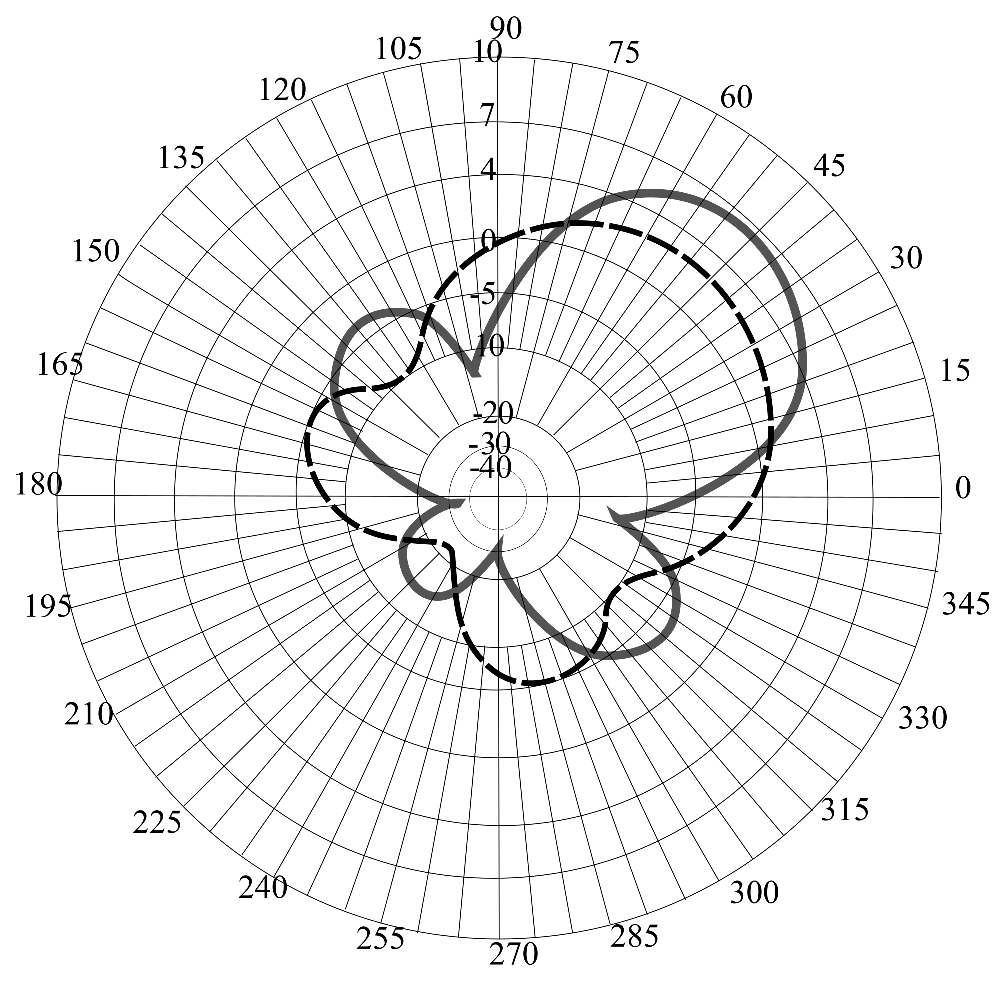
\includegraphics[width=0.5\linewidth]{BWE_comp.eps} }
    \vspace{0.7em}
    \caption{Горизонтальный план диаграммы направленности для решетки ШВИ 2x2 (пунктир) и ШВИ 3x3 (сплошная)}
    \label{ris:bve_comp}
\end{figure}

\begin{table}[!h]
\centering
\begin{tabular}{|l | l l | c c c | c c c|}
    \hline
    \textbf{ФАР} & \textbf{$M$} & \textbf{$M_{ne}$} & \textbf{$M_{f}$} & \textbf{$\mathcal{B}_{M_f}$} & \textbf{$\mathcal{L}_{M_f}$} & \textbf{$M_{y\approx0}$} & \textbf{$\mathcal{B}_{M_{y\approx0}}$} & \textbf{$\mathcal{L}_{M_{y\approx0}}$}\\
    \hline
    ШВИ 2x2 & 18368 & 4 & 1 & 1 & 1 & 4 & 4 & 4\\
    ШВД 2x2 & 7678  & 4 & 1 & 1 & 1 & 4 & 4 & 4\\
    СВД 2x2  & 523  & 1 & 1 & 1 & 1 & 1 & 1 & 1\\
    СВД 3x3  & 39  & 9 & 2 & 2 & 2 & 5 & 5 & 5\\
    СВД' 2x2  & 396  & 370 & 3 & 3 & 3 & 338 & 1000 & 1213\\
    СВД' 3x3  & 14  & 14 & 3 & 3 & 3 & 1 & 1 & 1\\
    ШВИ 3x3 & 1070  & 3 & 1 & 1 & 1 & 3 & 3 & 3 \\
    ШВД 3x3 & 41  & 4 & 4 & 4 & 4 & 1 & 1 & 1 \\
    Кольц. 8 & 124  & 9 & 2 & 2 & 2 & 9 & 9 & 9\\
    Кольц. 16 & 11  & 6 & 1 & 1 & 1& 6 & 6 & 6\\
    \hline
\end{tabular}
    \caption{Структура локальных оптимумов.}
    \label{tab:structure}
\end{table}

\begin{figure}
\centering
    \begin{minipage}[h]{0.8\linewidth}
            \center{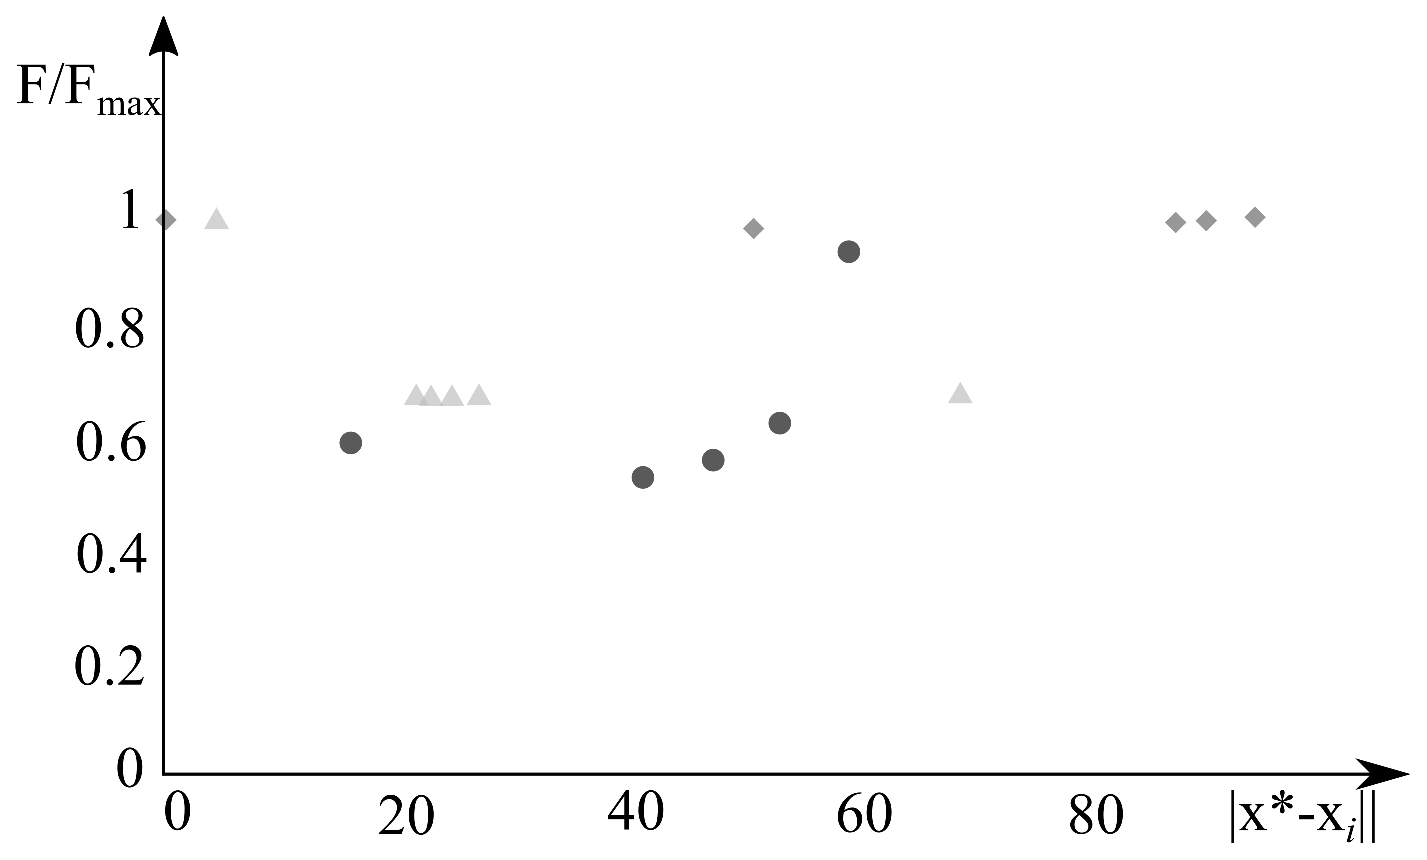
\includegraphics[width=0.9\linewidth]{fit_dist.eps}  \\ а) }
    \end{minipage}
    \begin{minipage}[h]{0.8\linewidth}
            \center{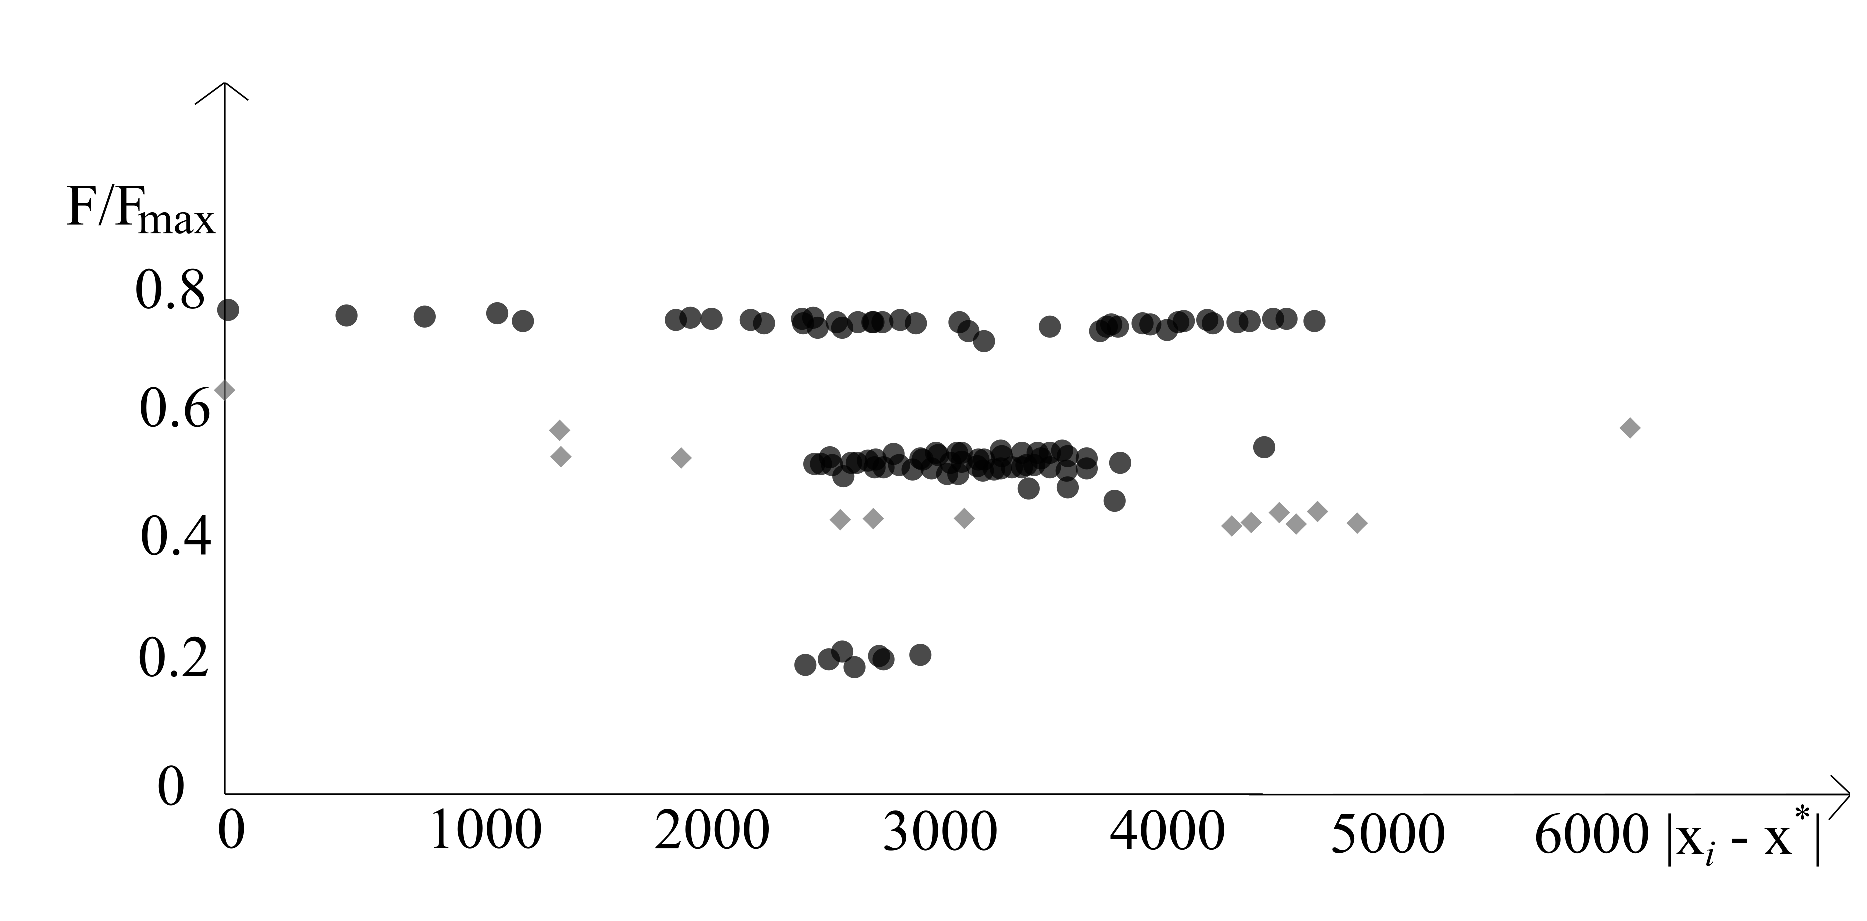
\includegraphics[width=0.9\linewidth]{fit_dist_2x2.eps}  \\ б) }
    \end{minipage}
    \vspace{0.7em}
    \caption{Структура множества найденных решений для задач ШВИ, ШВД, СВД (а) и СВД' (б)}
    \label{ris:fit_dist}
\end{figure}

Для оценки общего числа локальных оптимумов использовался метод переписи Шнабеля. Данный метод имеет применение в экологии и заключается в
выводе статистических оценок численности популяции на основе числа особей, помеченных в результате эксперимента, из популяции с неизменным
составом, где каждая особь имеет константную вероятность отлова. В~\cite{eremeev:confidence} предлагается адаптация такого метода для оценки числа локальных оптимумов. В таблице~\ref{tab:structure} приводится статистика по числу различных точек остановки (в пределах заданной точности) процедуры мультистарта в течение 1000~с. процессорного времени. Для каждого решения была применена процедура линеаризации задачи и проверки необходимых условий локальной оптимальности. Приемлемыми считались отличия целевой функции линеаризованной задачи от значения целевой функции, найденного градиентным методом менее чем на 1\%. Здесь {$M$} - число выполненных запусков за отведенное время, $M_{ne}$ - число групп решений, отличающихся не более чем на 10\% по каждой из координат, {$M_{f}$} - число групп значений целевой функции у таких неэквивалентных решений (с точностью до 10\%, приведенных в таблице~\ref{tab:results}). {$M_{y\approx0}$} - число групп решений, для которых были выполнены необходимые условия локальной оптимальности. $\mathcal{B}$ и $\mathcal{L}$ - оценка нижней границы и оценка максимального правдоподобия числа локальных оптимумов, рассчитанные по методу переписи Шнабеля. Доверительная вероятность для данного метода была выбрана равной 95\%. Оценки для числа решений с различными значениями целевой функции обозначены $\mathcal{B}_{M_f}$ и $\mathcal{L}_{M_f}$. Оценки для числа решений, для которых были выполнены необходимые условия локальной оптимальности, обозначены $\mathcal{B}_{M_{y\approx0}}$ и $\mathcal{L}_{M_{y\approx0}}$.
В случае СВД и СВД' конфигурации 5x5 в течение 1000~с градиентный метод не достиг решения, удовлетворяющего условию остановки, поэтому
данный результат не включен в таблицу~\ref{tab:structure}.

Как видно из таблицы, во всех экспериментах в некоторых запусках были найдены неразличимые с практической точки зрения решения. Для квадратных решеток ШВИ и ШВД было найдено по одному такому решению. Решетки кольцевой структуры и СВД'~2x2 имеют значительное разнообразие как по найденным векторам решений, так и по значениям целевой функции. Относительно решений, для которых были выполнены необходимые условия локальной оптимальности, можно сказать, что с большой вероятностью для задачи СВД'~2x2, были найдены далеко не все возможные решения. О решетке СВД'~3x3 известно, что градиентный подъем был остановлен в точке, не лежащей в окрестности решения, предоставляемого решателем BARON.

На рис.~\ref{ris:fit_dist} приведены диаграммы локальных оптимумов, где по оси ординат отложены значения целевой функции, а по оси
абсцисс - расстояние до лучшего известного решения. В случае а) точками обозначены результаты для кольцевых решеток, состоящих из 8 излучателей, ромбами - для кольцевых решеток, состоящих из 16 излучателей, пятиугольниками - для СВД~3x3. В случае б) точками обозначены результаты для СВД'~2x2, ромбами - для СВД'~3x3. Диаграмма показывает, что значения, соответствующие одному и тому же значению целевой функции, могут находиться достаточно далеко друг от друга, что позволяет сделать предположение о наличии неучтенных симметрий задачи (о множестве линейных симметрий задачи см. в~\cite{yurkov:symmetry}).

\begin{figure}[h]
    \centering
    \center{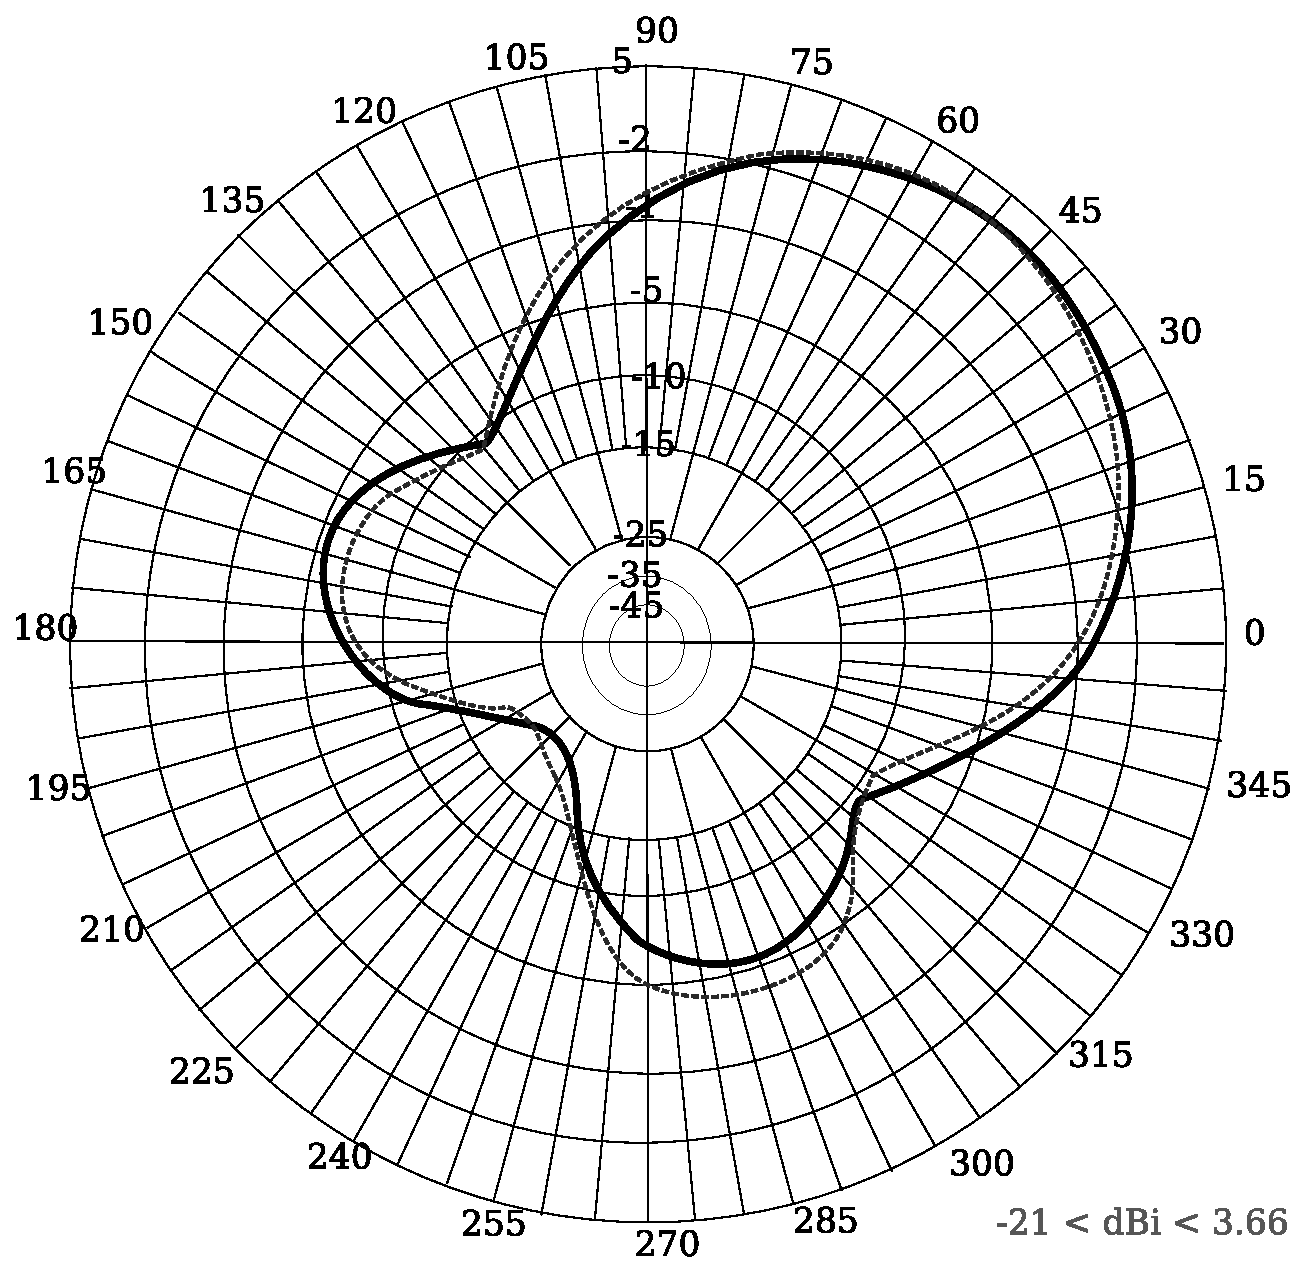
\includegraphics[width=0.5\linewidth]{stability.eps} }
    \vspace{0.7em}
    \caption{Диаграммы направленности для ШВИ~2x2 при оптимизации в направлении 70:45 (сплошная линия) и 70:50 (пунктир)}
    \label{ris:bve_stability}
\end{figure}
При анализе структуры локальных оптимумов может возникнуть вопрос об устойчивости решения по аргументу. В данной работе было проведено исследование изменения значения целевой функции при изменении оптимизируемого направления на малый угол. В рассмотрение принималось также изменение значения целевой функции при подстановки в исходную задачу решения, найденного для нового направления (для удобства вывода результата такая подстановка обозначена за P1), и наоборот - при подстановке в задачу для измененного направления решения, полученного для исходного направления (обозначается P2). Исследование проводилось на квадратных решетках, состоящих из 4-х и 9-и излучателей. Азимутальный и полярный угол менялись на $5^{\circ}$. Результаты приведены в таблице~\ref{tab:stability}
\begin{table}[!h]
\centering
\begin{tabular}{|c|c|c|c|c|c|c|c|}
    \hline
    \textbf{ФАР} & \textbf{Подстановка} & \textbf{70:45} & \textbf{75:45} & \textbf{65:45} & \textbf{70:50} & \textbf{75:40} & \textbf{65:50}\\
    \hline
    \multirow{3}{*}{ШВИ 2x2} & - & \multirow{3}{*}{138} & 125 & 138 & 137 & 137 & 125\\
    & P1 &  & 138 & 138 & 137 & 137 & 137\\
    & P2 &  & 125 & 138 & 136 & 136 & 123\\
    \hline
    \multirow{3}{*}{ШВИ 3x3} & - & \multirow{3}{*}{575} & 532 & 565 & 574 & 533 & 564\\
    & P1 &  & 574 & 572 & 560 & 558 & 557\\
    & P2 &  & 530 & 562 & 559 & 517 & 546\\
    \hline
    \multirow{3}{*}{ШВД 2x2} & - & \multirow{3}{*}{459} & 518 & 454 & 454 & 512 & 389\\
    & P1 &  & 458 & 459 & 457 & 456 & 389\\
    & P2 &  & 518 & 392 & 452 & 510 & 386\\
    \hline
    \multirow{3}{*}{ШВД 3x3} & - & \multirow{3}{*}{1501} & 1817 & 872 & 1015 & 1196 & 1198\\
    & P1 &  & 1506 & 1047 & 1000 & 1004 & 1448\\
    & P2 &  & 1774 & 1203 & 1450 & 1713 & 1162\\
    \hline
    \multirow{3}{*}{СВД 2x2} & - & \multirow{3}{*}{369} & 417 & 315 & 365 & 412 & 312\\
    & P1 &  & 368 & 369 & 367 & 366 & 367\\
    & P2 &  & 417 & 315 & 363 & 410 & 310\\
    \hline
    \multirow{3}{*}{СВД 3x3} & - & \multirow{3}{*}{1484} & 1789 & 1176 & 1459 & 1162 & 1753\\
    & P1 &  & 1475 & 1472 & 1446 & 1428 & 1444\\
    & P2 &  & 1782 & 1164 & 1427 & 1120 & 1713\\
    \hline
\end{tabular}
    \caption{Значения целевой функции при изменении оптимизируемого направления на малый угол.}
    \label{tab:stability}
\end{table}

Результаты исследования показывают~(см. Рис.\ref{ris:bve_stability}), что изменение направления оптимизации на малый угол соответствуют повороту исходной диаграммы направленности на этот угол.

Наличие большого количества решений, соответствующих одному и тому же значению целевой функции, приводит нас к исследованию групп симметрий. В~\cite{yurkov:symmetry} показано, что любой элемент группы непрерывных симметрий задачи~\ref{eq:task3} может быть описан в виде~\ref{eq:sunexp}.
\begin{equation}
\label{eq:sunexp}
Q=e^{\sum\limits_n a_n G_n} \, .
\end{equation}
где $a_n$ - вещественные числа, $G_n$ - генераторы. В качестве генераторов можно выбрать косо-симметричные матрицы, которые содержат над главной диагональю один единичный элемент, симметричный ему противоположный элемент и остальные нули.
Введем матрицу: $ {\textbf{H}}_{\Sigma} = \sum_{i} \textbf{H}_i,$ которая может быть представлена в виде конгруэнтного преобразования диагональной матрицы $D$:
$${\textbf{H}}_{\Sigma} = S^TDS,$$
Нахождение непрерывных групп симметрий сводится к решению задачи~\ref{eq:commutat2}.

\begin{equation}
\label{eq:commutat2}
\left\{
\begin{array}{l}
\displaystyle
\tilde{\textbf{H}}_i \left(\sum\limits_na_nG_n\right) =
\left(\sum\limits_na_nG_n\right)\tilde{\textbf{H}}_i \, , \\ \\
\displaystyle
\tilde{\textbf{G}} \left(\sum\limits_na_nG_n\right) = \left(\sum\limits_na_nG_n\right)\tilde{\textbf{G}} \, .
\end{array}
\right.
\end{equation}

\begin{equation}
\tilde{\textbf{G}}=\left(S^{-1}\right)^T \textbf{A} S^{-1} \, , \qquad
\tilde{\textbf{B}_i}=\left(S^{-1}\right)^T \textbf{B}_i S^{-1} \, , \ i=1,\dots,M.
\end{equation}

Вычислительный эксперимент состоит из следующих этапов:
\begin{enumerate}
  \item Обработка. На этом этапе возможная неточность данных нивелируется усреднением симметричных компонент матриц (матрицы $\textbf{G}$ и $\textbf{H}$ должны быть симметричны).
  \item %Normalization of matrices $B_i$.
  Преобразование $ {\textbf{H}}_{\Sigma} = \sum_{i} \textbf{H}_i$ к канонической форме используя метод Лагранжа для вычисления матриц~$S$ и $S^{-1} $.
  \item Применение метода Гаусса к системе линейных~(\ref{eq:commutat2}) для вычисления генераторов~$\hat{G}_n$.
\end{enumerate}

Следует отметить, что входные данные могут содержать некоторые погрешности, связанные с несимметричностью матриц $\textbf{G}$ и $\textbf{H}$, что может существенно повлиять на поиск непрерывных групп симметрий. Таким образом, на этапе~1, мы используем известные свойства задачи чтобы нивелировать влияние погрешности.
Также, в методе Гаусса на шаге 3, любые значения принимаются за 0 если их абсолютное значение меньше определенного порогового значения~$\Delta$, который является параметром алгоритма. Причина в том, что последовательное исключение переменных из уравнений, выполняемое методом Лагранжа с представлением вещественных чисел с плавающей запятой, не может гарантировать идеальную точность.
В результате некоторые линейно зависимые строки матрицы не могут быть исключены, что может привести к неверному результату.
%To eliminate this effect, a threshold error is introduced.
Большое значение порога~$\Delta$ может привести к вырожденности задачи, тогда как слишком малое значение~$\Delta$ не позволит выявить линейные зависимости.
В данном эксперименте, $\Delta$ изменялось от $ 10^{-4} $ до $ 10^{-12} $. В данном диапазоне для каждого рассмотренного частного случая задачи, не было получено различий в полученных решениях.

%\subsection{Optimization of the Excitation of Antenna Arrays}

Описанная процедура нахождения непрерывных групп симметрий применяется к примерам, описанным во второй главе. Для всех рассмотренных задач было выявлено только наличие фазовой симметрии. Возможно, множественность решений объясняется наличием дискретных симметрий. Выявление дискретных симметрий является объектом дальнейших исследований.

Как было показано выше, градиентный метод может предоставить решение, не являющийся локальным оптимумом, если целевая функция слабо изменяется в окрестности текущей точки. Алгоритм дифференциальной эволюции не подвержен такому поведению.
Эксперименты показывают, что в целом эволюция популяции соответствует динамике случайного облака точек, движущегося как целое вдоль рельефа оптимизируемой функции, повторяя его характерные особенности. В случае попадания в овраг «облако» принимает форму этого оврага и распределение точек становится таким, что математическое ожидание разности двух случайных векторов оказывается направленным вдоль длинной стороны оврага. Это обеспечивает быстрое движение вдоль узких вытянутых оврагов, тогда как для градиентных методов в аналогичных условиях характерно колебательная динамика «от стенки к стенке». Приведенные эвристические соображения иллюстрируют наиболее важную и привлекательную особенность алгоритма ДЭ — способность динамически моделировать особенности рельефа оптимизируемой функции. Именно этим объясняется замечательная способность алгоритма быстро проходить сложные овраги, обеспечивая эффективность даже в случае сложного рельефа.

Кратко опишем идею алгоритма ДЭ. В начале происходит генерация популяции. Если нет дополнительной информации, такая популяция особи популяции генерируются случайным образом с равномерным распределением. Затем, пока все особи не сойдутся в одной точке, каждая особь подвергается мутации путем присваивания ей признаков другой особи. Процедура, определяющая, в какой степени признаки других особей участвуют в эволюции конкретной особи является параметром алгоритма. Далее происходит сравнение значений целевой функции мутировавшей особи со значением целевой функции исходной особи. Выживает особь с лучшим значением целевой функции.

Данный алгоритм хорошо поддается модификации для запуска в параллельных потоках. В этом случае, на очередной итерации алгоритма выбирается некоторый набор особей, эволюция каждой из которых на данной итерации происходит независимо от эволюции другой. В данной работе был предложен вариант реализации алгоритма дифференциальной эволюции, адаптированный для запуска на графическом устройстве. Использование алгоритма ДЭ позволило достичь решения с целевой функцией $\tilde{F} = 253$ для задачи СВД'~2x2.

\underline{\textbf{Третья глава}} посвящена исследованию ФАР в различных условиях.

На практике использование высоко симметричных ФАР вызывает особый интерес из следующих соображений: измерение матрицы сопротивлений является тривиальной задачей, в то время как измерение парциальных полей требует большое количество приемников для всех возможных направлений излучения. Использование высокосимметричных ФАР позволяет выполнить расчеты для одного направления и затем легко адаптировать их для других симметричных направлений. Другой особенностью, влияющей на результаты моделирования является наличие потерь в земле (см.~\cite{yurkov:groundloss}). Чтобы ослабить этот эффект, антенные системы с противовесами подняты над землей на 2 м.

В данной главе мы изучаем, как изменяется общий коэффициент усиления с ростом радиочастоты и плотности системы противовесов. Общий коэффициент усиления является суммой частичных коэффициентов усиления в  двух ортогональных поляризациях. Плотность системы противовесов определяется числом продольных и поперечных проводов, относящихся к одному и тому же излучателю. Частота изменяется от 5 до 30 МГц. Вычисления производились на решетках ШВИ, состоящих из 8 излучателей. Для расчета матрицы сопротивлений и матрицы излучений использовался пакет моделирования антенных систем NEC2~\cite{bruke:nec2}.

Для проведения вычислительного эксперимента использовался решатель BARON в пакете GAMS, поскольку, в основном он деонстрирует лучшие результаты по сравнению с градиентным подъемом. Результаты оптимизации направленности решетки сравниваются с коэффициентом усиления одиночного излучателя, установленного в центре такой же системы противовесов. Плотность системы противовесов обозначается в формате $long:trans$, где $long$ - число продольных проводов, относящихся к одному излучателю, а $trans$ - поперечных. Высота каждого ШВИ - 15м. В качестве направления оптимизации выбирается $70^{\circ}$ полярного угла и $45^{\circ}$ азимутального угла в сферических координатах.

\begin{figure}
\center{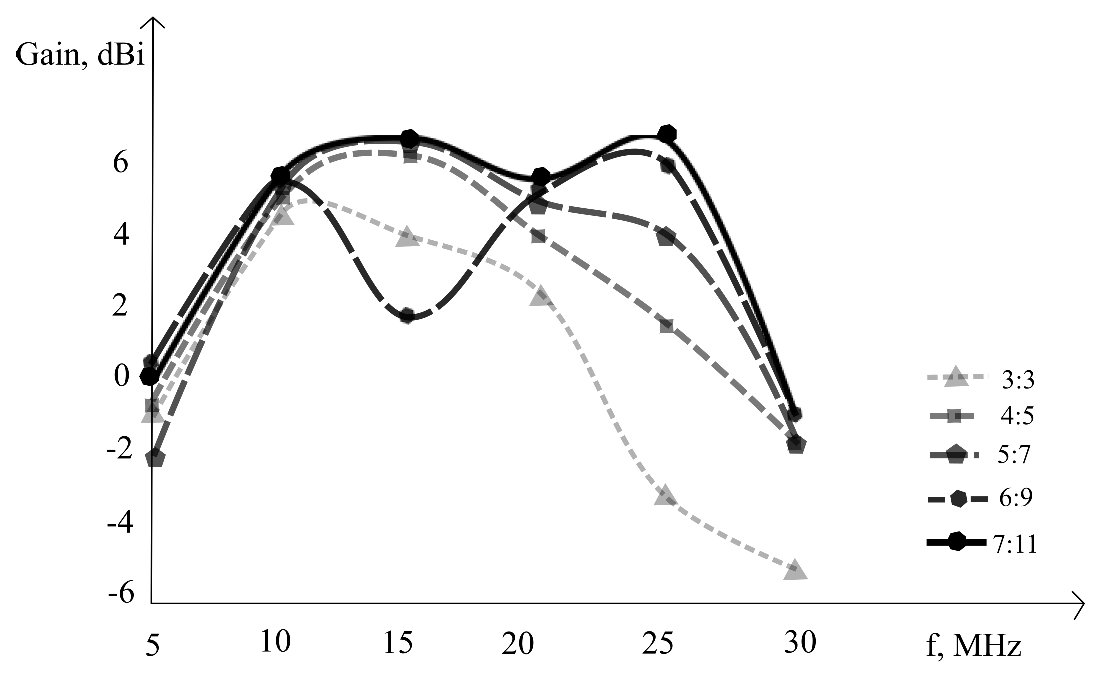
\includegraphics[width=0.8\linewidth]{ring_f__paa_gains.eps}}
\caption{Зависимость от частоты общего коэффициента усиления ФАР при оптимизации в направлении 70:45}
\label{ris:paa_gains}
\end{figure}

На рис.~\ref{ris:paa_gains} показано, как изменяется коэффициент усиления с ростом радиочастоты. Мы можем наблюдать, что при значениях частоты 5 и 30 МГц решетка оптимизируется довольно плохо. Также можно увидеть, что, в основном, увеличение плотности системы противовесов приводит к росту коэффициента усиления. Единственное исключение - решетка с плотностью системы противовесов $6:9$ на частоте 15МГц, где наблюдается неожиданное падение коэффициента усиления. Такое поведение может быть объяснено тем, что BARON не достиг глобалного оптимума.

\begin{figure}
\center{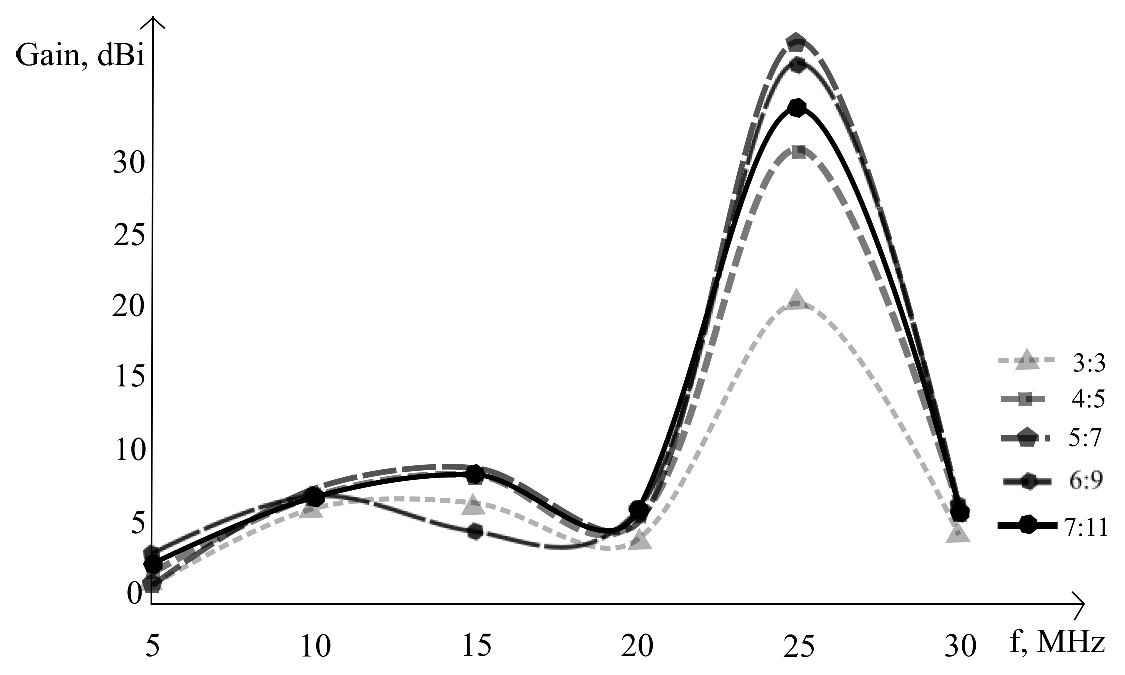
\includegraphics[width=0.8\linewidth]{ring_f_gains.eps}}
\caption{Сравнение коэффициентов усиления ФАР и одиночного излучателя}
\label{ris:all_gains}
\end{figure}

На рис.~\ref{ris:all_gains} показано, как изменяется разница коэффициентов усиления ФАР и одиночного излучателя с ростом частоты. Заметным результатом здесь является то, что на частоте 25МГц усиление ФАР существенно больше усиления одиночного излучателя. Объяснение этого эфффекта будет приведено далее при сравнении диаграмм направленности. При 5МГц усиление ФАР существенно не превосходит усиление одиночного излучателя, однако, уже на 10МГц разница возрастает до 7.53дБ. Даже при 30МГц, где ФАР не оптимизируется хорошо, разница с одиночным излучателем составляет 6.63дБ в лучшем случае и 4.84дБ в худшем.

Далее будут рассмотрены диаграммы направленности ФАР с плотностью противовесов $5:7$ как один из наиболее типичных результатов.

\begin{figure}
\begin{minipage}[h]{0.49\linewidth}
\center{\includegraphics[width=1\linewidth]{r8_1_5_5x7.png} \\ а)}
\end{minipage}
\hfill
\begin{minipage}[h]{0.49\linewidth}
\center{\includegraphics[width=1\linewidth]{r8_5_5x7.png} \\ б)}
\end{minipage}
\caption{Вертикальный план диаграммы направленности одиночного излучателя (а) и ФАР 5:7 (б) при 5МГц}
\label{ris:5MHz}
\end{figure}

При частоте 5МГц (см Рис.~\ref{ris:5MHz}) мы можем наблюдать, что максимум усиления в случае ФАР приходится на $70^{\circ}$ и превосходит соответствующее значение одиночного излучателя на 1.33~дБ. Использование ФАР с плотностью системы противовесов 6:9 позволяет увеличить этот параметр до 3.14~дБ.

\begin{figure}
\begin{minipage}[h]{0.49\linewidth}
\center{\includegraphics[width=1\linewidth]{r8_1_10_5x7.png} \\ а)}
\end{minipage}
\hfill
\begin{minipage}[h]{0.49\linewidth}
\center{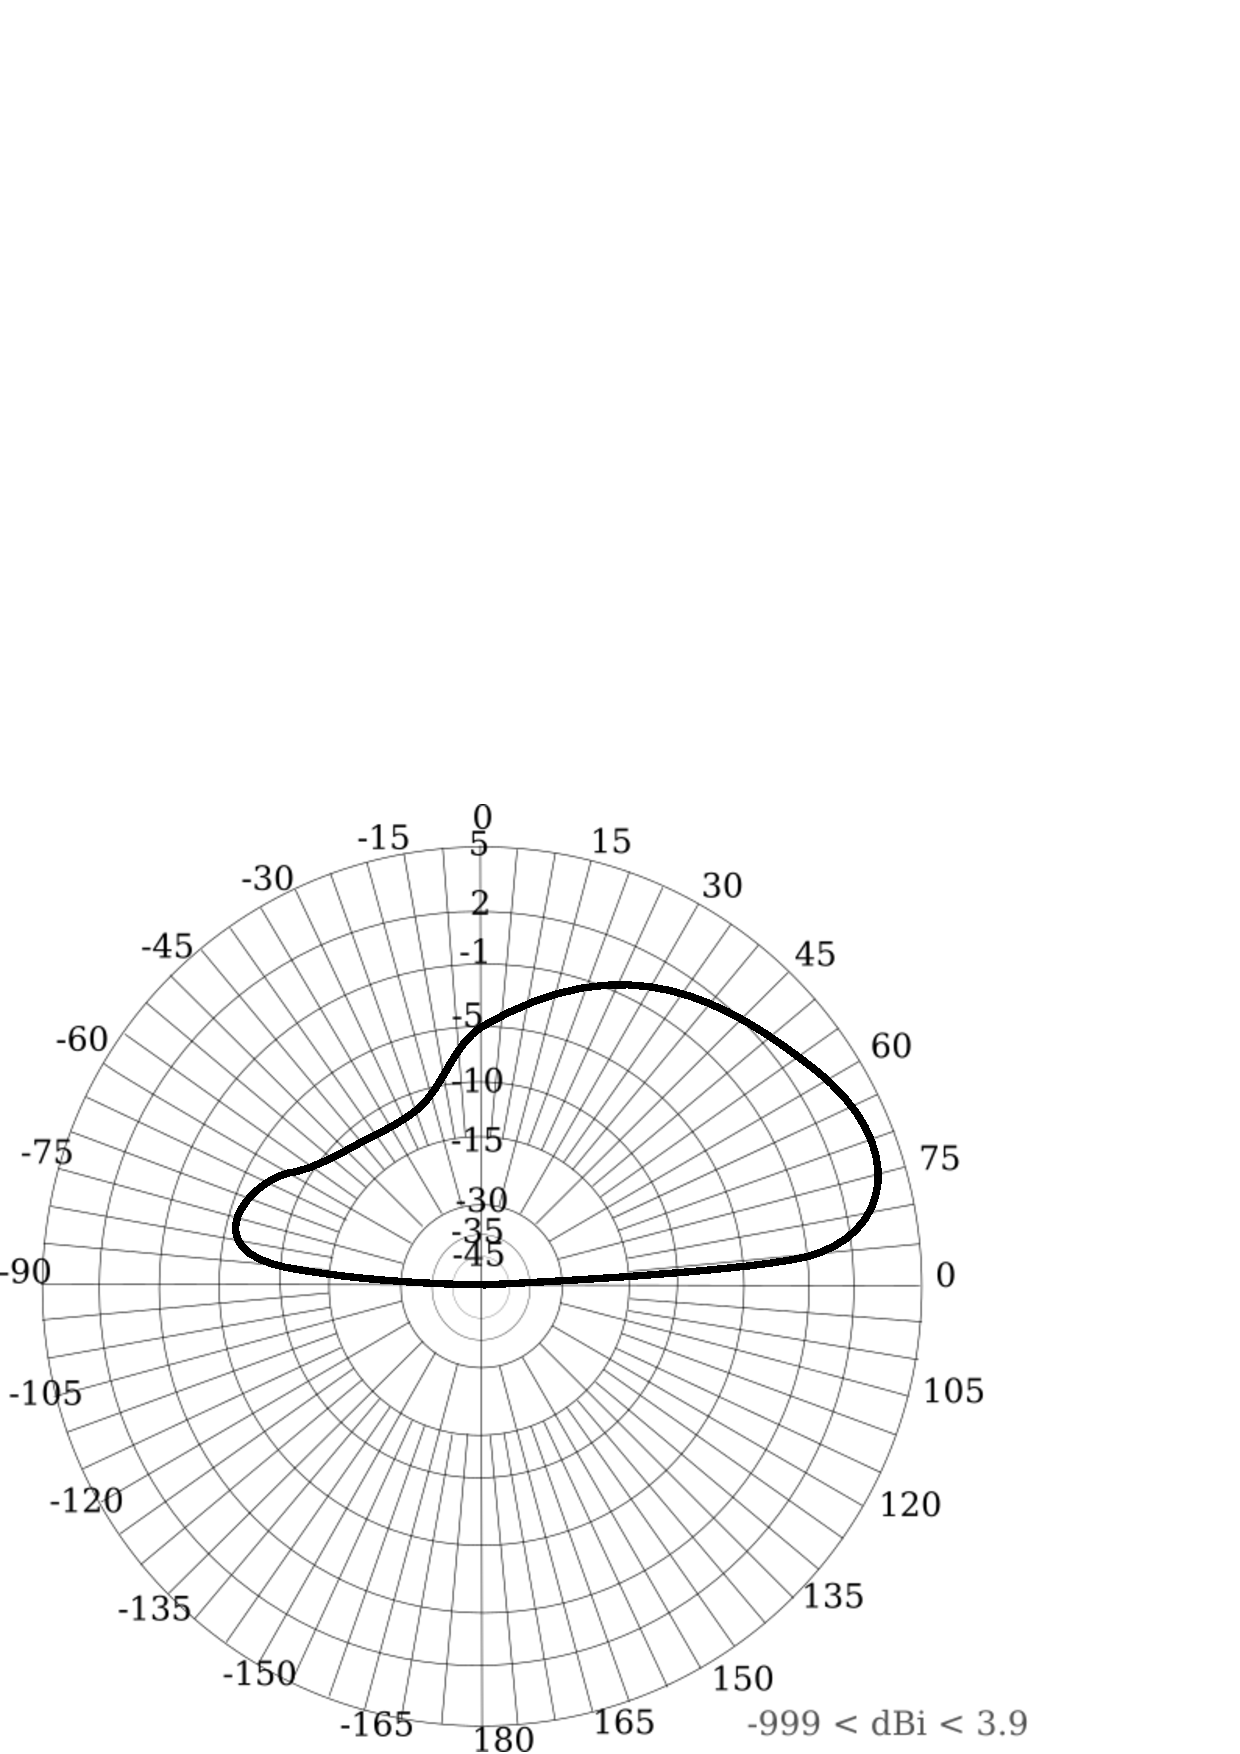
\includegraphics[width=1\linewidth]{r8_10_5x7.png} \\ б)}
\end{minipage}
\caption{Вертикальный план диаграммы направленности одиночного излучателя (а) и ФАР 5:7 (б) при 10МГц}
\label{ris:10MHz}
\end{figure}

Результат оптимизации более заметен при частоте 10МГц~(см~Рис.~\ref{ris:10MHz}): задний лепесток существенно меньше и разница усиления к одиночному излучателю достигает примерно~8~дБ. Похожие результаты наблюдаются при частоте~15МГц.

\begin{figure}
\begin{minipage}[h]{0.49\linewidth}
\center{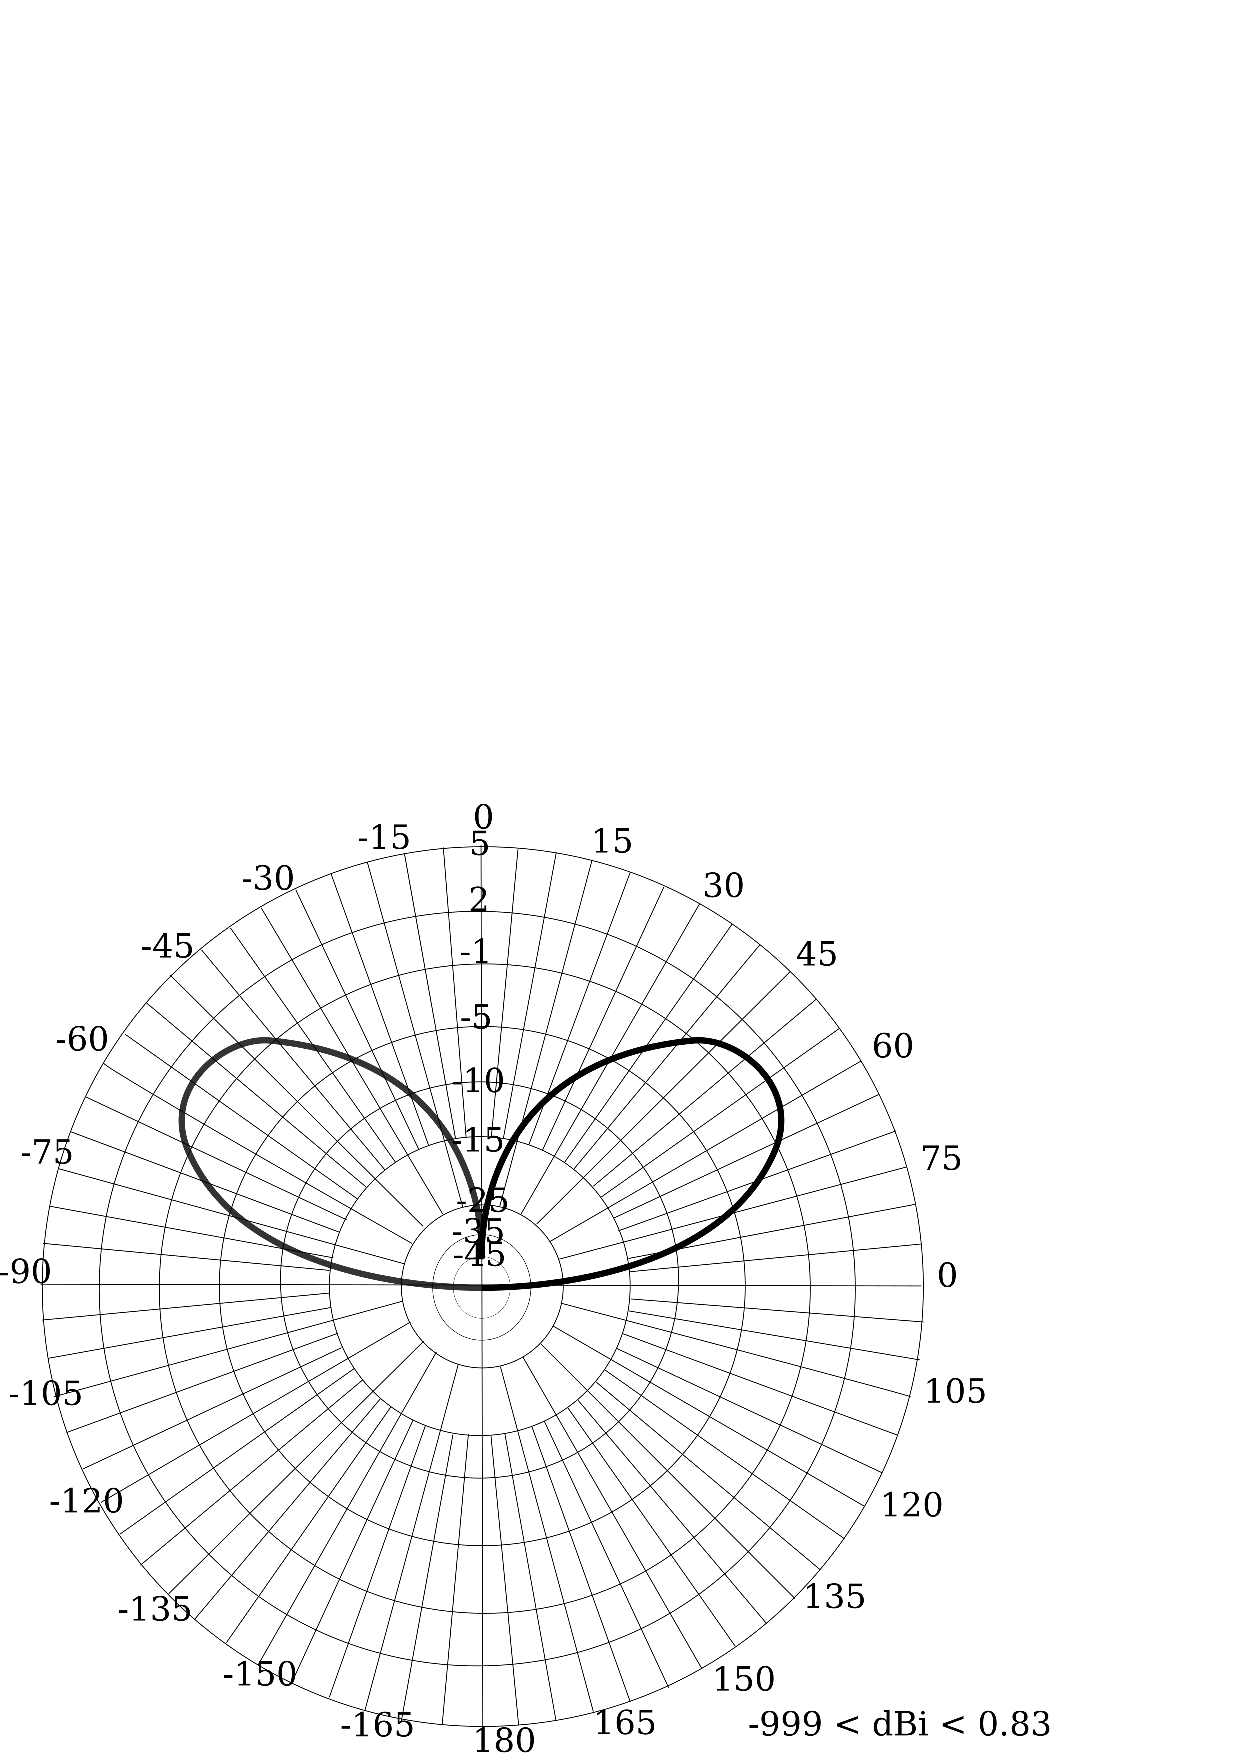
\includegraphics[width=1\linewidth]{r8_1_20_5x7.png} \\ а)}
\end{minipage}
\hfill
\begin{minipage}[h]{0.49\linewidth}
\center{\includegraphics[width=1\linewidth]{r8_20_5x7.png} \\ б)}
\end{minipage}
\caption{Вертикальный план диаграммы направленности одиночного излучателя (a) и ФАР 5:7 (b) при 20МГц}
\label{ris:f20mhs}
\end{figure}

При 20МГц мы можем наблюдать, что как в случае одиночного излучателя, так и в случае ФАР, коэффициент усиления падает по отношению к результату при 15МГц~(см~Рис.~\ref{ris:paa_gains}). Диаграмма направленности изображена на рис.~\ref{ris:f20mhs}.

\begin{figure}
\begin{minipage}[h]{0.49\linewidth}
\center{\includegraphics[width=1\linewidth]{r8_1_25_5x7.png} \\ а)}
\end{minipage}
\hfill
\begin{minipage}[h]{0.49\linewidth}
\center{\includegraphics[width=1\linewidth]{r8_25_5x7.png} \\ б)}
\end{minipage}
\caption{Вертикальный план диаграммы направленности одиночного излучателя (а) и ФАР 5:7 (б) при 25МГц}
\label{ris:f25mhs}
\end{figure}

Интересный результат наблюдается при 25МГц (см~Рис.~\ref{ris:f25mhs}), где усиление ФАР существенно больше усиления одиночного излучателя. Сравнение их диаграмм направленности показывает, что одиночный излучатель довольно плохо излучает в направлении оптимизации, тогда как ФАР имеет максимум излучения в этом направлении. Предположительно, такой эффект был получен вследствие учета взаимного влияния. Согласно~(\ref{eq:A}), если пренебречь взаимным влиянием излучателей, плотность мощности $F$ будет максимальна тогда, когда комплексные амплитуды парциальных полей будут синфазны. Для проверки гипотезы о необходимости учета взаимного влияния в данной работе производилось сравнение диаграмм направленности решеток разных конфигураций после математической оптимизации их направленности в заданном направлении согласно модели~(\ref{eq:task3}) с соответствующими диаграммами одиночного излучателя и со случаем фазирования решетки без учета взаимного влияния (далее – простое фазирование).

Для проведения вычислительного эксперимента использовался решатель BARON в пакете GAMS, поскольку, как правило, он обеспечивает бо́льшую точность решений по сравнению с градиентным подъемом [A1]. Высота каждого ШВИ равна 15~м. Длина плеча симметричных излучателей также равна 15~м. Направление оптимизации по умолчанию было установлено на $70^{\circ}$ полярного угла и $45^{\circ}$ азимутального угла в сферических координатах. Для некоторых экспериментов было проведено дополнительное исследование при $85^{\circ}$ полярного угла.


\begin{figure}
    \begin{minipage}[h]{0.49\linewidth}
        \center{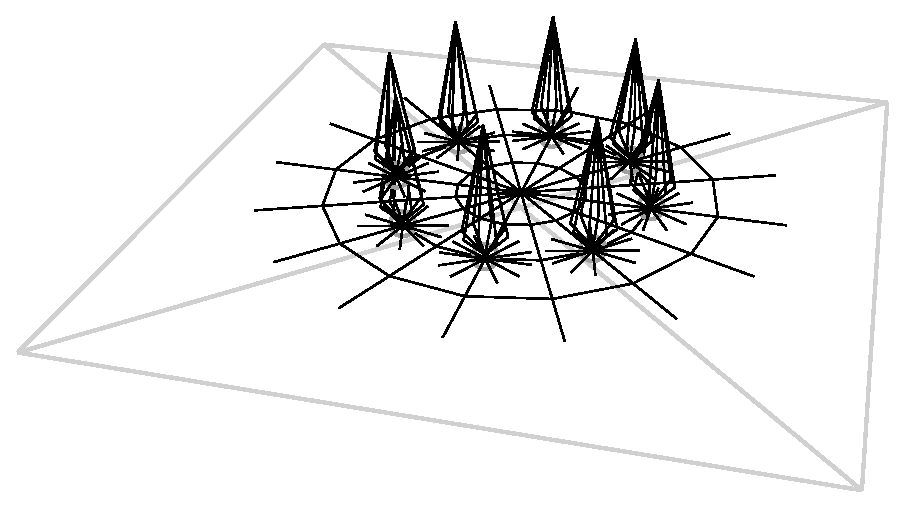
\includegraphics[width=0.8\linewidth]{r_bve_w.eps} \\ а)}
    \end{minipage}
    \hfill
    \begin{minipage}[h]{0.49\linewidth}
        \center{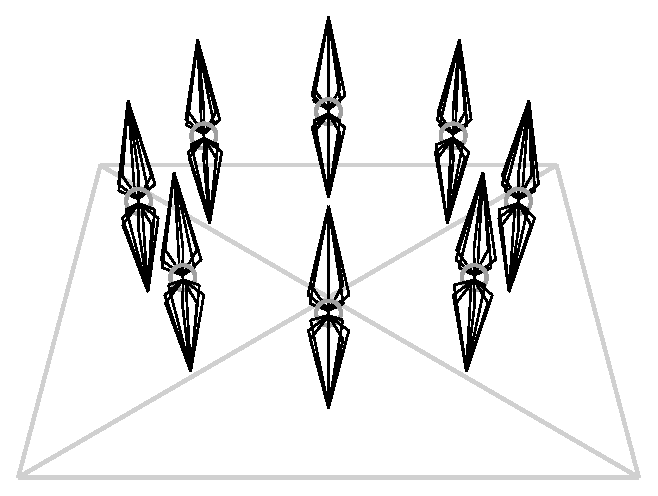
\includegraphics[width=0.6\linewidth]{r_bvd.eps} \\ б)}
    \end{minipage}
    \begin{minipage}[h]{1\linewidth}
        \center{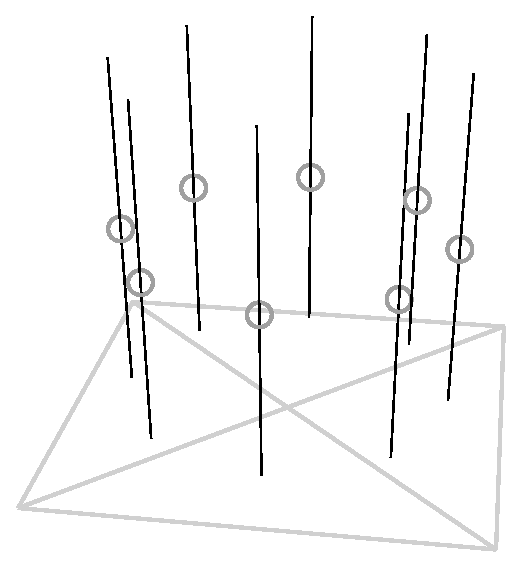
\includegraphics[width=0.25\linewidth]{r_svd.eps} \\ в)}
    \end{minipage}
    \caption{ФАР кольцевой структуры: ШВИ (а) ШВД (б) и СВД (в)}
    \label{pic:r_paas}
\end{figure}

Для решеток ШВИ~(см.~Рис.~\ref{pic:r_paas},~а.) производилось сравнение диаграмм направленности при варьировании расстояния центра излучателя до центра решетки (от~7 до 80~м.), длины радиальных противовесов (от 3 до 20 м.) и присутствия или отсутствия общей системы противовесов. Диаграммы направленности при этом имели различную форму, однако, качественно различие между коэффициентами усиления всегда сохранялось ~(см.~Рис.~\ref{pic:r_bve_result}): результат оптимизации не дает значимого преимущества перед простым фазированием.

\begin{figure}
\begin{minipage}[h]{0.49\linewidth}
\center{\includegraphics[width=1\linewidth]{r_bve_15_results_h.png} \\ а)}
\end{minipage}
\hfill
\begin{minipage}[h]{0.49\linewidth}
\center{\includegraphics[width=1\linewidth]{r_bve_15_results_v.png} \\ б)}
\end{minipage}
\caption{Горизонтальный (а) и вертикальный (б) план диаграммы направленности ШВИ при расстоянии от центра излучателя до центра решетки 15 м. и длиной радиальных противовесов 5 м. Пунктирной линией обозначено усиление одиночного излучателя, штрихпунктирной – простое фазирование, сплошной – решение задачи мат. программирования.}
\label{pic:r_bve_result}
\end{figure}

Для ШВД~(см.~Рис.~\ref{pic:r_paas},~б.) производилось исследование диаграмм направленности при варьировании расстояния центра излучателя до центра решетки от~5 до 50~м. В большинстве случаев, использование решения задачи математического программирования не давало существенного преимущества перед простым фазированием~(см.~Рис.~\ref{pic:r_bvd_result_0}). Тем не менее, при расстоянии между центром излучателя и центром решетки равным 20~м. это различие составило около 4~дБ~(см.~Рис.~\ref{pic:r_bvd_result}).

\begin{figure}
\begin{minipage}[h]{0.49\linewidth}
\center{\includegraphics[width=1\linewidth]{r_bvd_30_results_h.png} \\ а)}
\end{minipage}
\hfill
\begin{minipage}[h]{0.49\linewidth}
\center{\includegraphics[width=1\linewidth]{r_bvd_30_results_v.png} \\ б)}
\end{minipage}
\caption{Рис. 3. Горизонтальный (а) и вертикальный (б) план диаграммы направленности ШВД при расстоянии от центра излучателя до центра решетки 30 м. Пунктирной линией обозначено усиление одиночного излучателя, штрихпунктирной – простое фазирование, сплошной – решение задачи мат. программирования.}
\label{pic:r_bvd_result_0}
\end{figure}

\begin{figure}
\begin{minipage}[h]{0.49\linewidth}
\center{\includegraphics[width=1\linewidth]{r_bvd_20_results_h.png} \\ а)}
\end{minipage}
\hfill
\begin{minipage}[h]{0.49\linewidth}
\center{\includegraphics[width=1\linewidth]{r_bvd_20_results_v.png} \\ б)}
\end{minipage}
\caption{Горизонтальный (а) и вертикальный (б) план диаграммы направленности ШВД при расстоянии от центра излучателя до центра решетки 20 м. Пунктирной линией обозначено усиление одиночного излучателя, штрихпунктирной – простое фазирование, сплошной – решение задачи мат. программирования.}
\label{pic:r_bvd_result}
\end{figure}

Аналогичные результаты были получены и для решетки~(см.~Рис.~\ref{pic:r_paas},~в.). При оптимизации в направлении полярного угла равном $70^{\circ}$ при варьировании расстояния от центра излучателя до центра решетки от~35 до 37~м. разница между коэффициентом усиления решения задачи математического программирования и усилением простого фазирования также достигала 4~дБ~(см.~Рис.~\ref{pic:r_svd_result}).  При оптимизации в направлении полярного угла равном $85^{\circ}$ при варьировании расстояния от центра излучателя до центра решетки от 25 до 29~м. эта разница достигала 5~дБ.~(см.~Рис.~\ref{pic:r_svd_result_1}).

\begin{figure}
\begin{minipage}[h]{0.49\linewidth}
\center{\includegraphics[width=1\linewidth]{r_svd_37_results_h.png} \\ а)}
\end{minipage}
\hfill
\begin{minipage}[h]{0.49\linewidth}
\center{\includegraphics[width=1\linewidth]{r_svd_37_results_v.png} \\ б)}
\end{minipage}
\caption{Горизонтальный (а) и вертикальный (б) план диаграммы направленности СВД при расстоянии от центра излучателя до центра решетки 37 м. Пунктирной линией обозначено усиление одиночного излучателя, штрихпунктирной – простое фазирование, сплошной – решение задачи мат. программирования.}
\label{pic:r_svd_result}
\end{figure}

\begin{figure}
\begin{minipage}[h]{0.49\linewidth}
\center{\includegraphics[width=1\linewidth]{r_svd_25_results_h.png} \\ а)}
\end{minipage}
\hfill
\begin{minipage}[h]{0.49\linewidth}
\center{\includegraphics[width=1\linewidth]{r_svd_25_results_v.png} \\ б)}
\end{minipage}
\caption{Горизонтальный (а) и вертикальный (б) план диаграммы направленности СВД при расстоянии от центра излучателя до центра решетки 25 м, полученные для $85^{\circ}$ полярного угла. Пунктирной линией обозначено усиление одиночного излучателя, штрихпунктирной – простое фазирование, сплошной – решение задачи мат. программирования.}
\label{pic:r_svd_result_1}
\end{figure}

В \underline{\textbf{четвертой главе}} приведено разработанного программного комплекса. Для проведения вычислительных экспериментов был разработан интерпретатор <<Expi>> и его графическая оболочка <<ExpiIDE>>.

Формат языка <<Expi>> позволяет в декларативной форме объявлять правила построения моделей и задавать параметры запуска экспериментов. Например, рассмотрим проведение эксперимента по исследованию эффекта взаимного влияния для кольцевых ШВД. Для этого потребуется описать <<каплеобразный>> излучатель, который состоит из 8-ми <<колен>>. Для построения <<колена>> нужно провести проводник через три точки.
\begin{lstlisting}
def knees = 8
def height = 15
def kneeWidth = 2.5

def Drop {
   def step = 2 * pi / knees
   for angle from 0 to 2 * pi by step {
      rotate around z by angle
      (0, 0, 0) -> 
      (kneeWidth, 0, kneeWidth) -> 
      (0, 0, height)
   }
}

\end{lstlisting}   

В приведенном листинге с помощью команды \lstinline$def varName = value$ объявляются переменные. Здесь объявляются следующие переменные:\\
\lstinline$def knees = 8$: количество колен в излучателе, \\ \lstinline$def height = 15$: высота <<каплеобразного>> излучателя, \\ \lstinline$def kneeWidth = 2.5$: расстояние, на которое выносится <<колено>> излучателя. \\
Команда \lstinline$def GroupName {}$ позволяет объявлять группы инструкций для их последующего использования.
Внутри группы \lstinline$Drop$ вычисляется угол между двумя соседними <<коленами>> и запускается цикл по кругу: \lstinline$for angle from 0 to 2 * pi by step {}$. Внутри цикла объявляется поворот всех последующих инструкций на заданный угол: \lstinline$rotate around z by angle$ и проводится провод через три точки колена: \lstinline$(0, 0, 0) -> (kneeWidth, 0, kneeWidth) -> (0, 0, height)$.

Далее требуется сформировать излучатель ШВД, который представляет собой два противоположно направленных <<каплеобразных>> излучателя, соединенных коротким проводом к которому подключен генератор.

\begin{lstlisting}
def base = 0.5

def BVD {
   (0, 0, -base / 2) ~1v~ (0, 0, base / 2)
   translate z to base / 2
   Drop
   rotate around x by pi
   Drop
}

\end{lstlisting}   

Для подключения генератора в сегмент провода нужно вместо инструкции \lstinline$->$ указать \lstinline$~voltageOrCurrent~$. В качестве единицы измерения можно указывать как вольты, так и амперы, причем как в вещественной, так и в комплексной форме.
Итак, мы провели короткий проводник с подключенным генератором: \lstinline$(0, 0, -base / 2) ~1v~ (0, 0, base / 2)$. Теперь поднимем все последующие инструкции так, чтобы начало координат приходилось на конец этого проводника: \lstinline$translate z to base / 2$ и установим туда <<каплеобразный>> излучатель: \lstinline$Drop$. Теперь развернем последующие инструкции на $180^{\circ}$: \lstinline$rotate around x by pi$ и установим излучатель в противоположном направлении: \lstinline$Drop$.

Остается только установить излучатели в решетку.

\begin{lstlisting}
def count = 8

def PAA {
    def step = 2 * pi / count
    for angle from 0 to 2 * pi by step {
        rotate around z by angle
        translate x to radius
        BVD
    }
}

\end{lstlisting} 

Переменная radius является динамической и будет задана в настройках эксперимента. Все остальные языковые конструкции, приведенные в данном листинге уже описаны выше.

Для проведения вычислительного эксперимента требуется экспортировать требуемые инструкции в формат NEC.

\begin{lstlisting}
def ExportPAA {
    export nec (n: 'r_bvd_${radius}.nec', f: 5, g: 'real') {
        PAA
    }
}
\end{lstlisting}

При этом, команде \lstinline$nec$ требуется передать имя файла, частоту и пресет параметров земли. Обратите внимание, что имя файла может быть параметризованно, что позволит генерировать файлы с отличающимися именами в серии экспериментов. Для проведения серии экспериментов достаточно запустить цикл с варьированием требуемого параметра, экспортировать nec файл и выполнить команду \lstinline$solve paa$.

\begin{lstlisting}
for radius from 3 to 50 by 2 {
    ExportPAA
    solve paa (
        theta: 70, phi: 45,
        nec: 'r_bvd_${radius}.nec',
        compare: 'bvd-1.nec',
        package: 'GAMS', solver: 'QCP=BARON'
    )
}
\end{lstlisting}

Данная команда принимает направление оптимизации в параметрах \lstinline$theta$ и \lstinline$phi$, имя nec файла, содержащего модель решетки, имя nec файла, содержащего модель антенны, с которой требуется произвести сравнение диаграмм, название оптимизационного пакета и решателя. В <<Expi>> уже встроен интерфейс для работы с пакетом GAMS. Однако, для его правильной работы, требуется установить путь до исполняемого пакета в переменных среды операционной системы. Имеется возможность использования любого пользовательского пакета. Для этого, исполняемый файл пакета должен реализовывать следующий вызов из командной строки:

\begin{lstlisting}
package solver --input problem.bin --output solution.bin
\end{lstlisting}

В файле \lstinline$problem.bin$ должны находится входные данные задачи оптимизации в бинарном формате, в файл \lstinline$solution.bin$ должно выводится полученное решение в бинарном формате. Исполняемый файл пакета можно расположить в директории исполняемого файла <<Expi>> или же указать путь в переменных среды операционной системы.

Графическая оболочка <<ExpiIDE>> представляет собой файловый инспектор с возможностью редактировать и запускать файлы экспериментов exp, просматривать и экспортировать диаграммы направленности и геометрию антенных систем~(см. Рис.~\ref{ris:expi_ide}).
\begin{figure}[h]
    \centering
    \center{\includegraphics[width=1\linewidth]{expi_ide.png} }
    \vspace{0.7em}
    \caption{Графический интерфейс ExpiIDE}
    \label{ris:expi_ide}
\end{figure}

\FloatBarrier
\pdfbookmark{Заключение}{conclusion}                                  % Закладка pdf
В \underline{\textbf{заключении}} приведены основные результаты работы, которые заключаются в следующем:
%% Согласно ГОСТ Р 7.0.11-2011:
%% 5.3.3 В заключении диссертации излагают итоги выполненного исследования, рекомендации, перспективы дальнейшей разработки темы.
%% 9.2.3 В заключении автореферата диссертации излагают итоги данного исследования, рекомендации и перспективы дальнейшей разработки темы.
\begin{enumerate}
\item Предложена модификация градиентного метода, учитывающая специфику задачи оптимизации фаз и амплитуд ФАР. 
Решения, полученные этим алгоритмом на тестовых задачах, отличались от результатов коммерческого решателя не более, чем на 1\% по целевой функции.
\item Предложена многопроцессорная модификация алгоритма дифференциальной эволюции в комбинации с градиентным алгоритмом. Решения, полученные этим алгоритмом, на тестовых задачах наибольшей размерности оказались точнее, чем результаты коммерческого решателя.   
  \item Методами линейной алгебры выявлена одномерная непрерывная группа симметрий в задаче оптимизации фаз и амплитуд ФАР. Все тестовые задачи оказались симметричны только относительно равного сдвига фаз во всех излучателях.
  \item В ходе вычислительного эксперимента показано, что задача оптимизации фаз и амплитуд фазированной антенной решетки имеет многочисленные локальные оптимумы, многие из которых совпадают по целевой функции, однако не эквивалентны между собой относительно равного сдвига фаз во всех излучателях.
%В текущей работе была рассмотрена постановка задачи оптимизации направленности излучения антенной системы, представленной в виде регулярной решетки излучателей. Для данной задачи была разработана модель квадратичного программирования в вещественных числах. Произведено сравнение результатов разработанных алгоритмов в вычислительном эксперименте.
  \item Выявлены ситуации, в которых коэффициент усиления, соответствующий решению задачи квадратичной оптимизации, имеет существенное преимущество (до 5 дб) перед коэффициентом усиления, получаемым стандартным методом простого фазирования. 
\end{enumerate}


\pdfbookmark{Литература}{bibliography}                                

\ifdefmacro{\microtypesetup}{\microtypesetup{protrusion=false}}{} % не рекомендуется применять пакет микротипографики к автоматически генерируемому списку литературы
\urlstyle{rm}                               % ссылки URL обычным шрифтом
\ifnumequal{\value{bibliosel}}{0}{% Встроенная реализация с загрузкой файла через движок bibtex8
    \renewcommand{\bibname}{\large \bibtitleauthor}
    \nocite{*}
    \insertbiblioauthor           % Подключаем Bib-базы
    %\insertbiblioexternal   % !!! bibtex не умеет работать с несколькими библиографиями !!!
}{% Реализация пакетом biblatex через движок biber
    % Цитирования.
    %  * Порядок перечисления определяет порядок в библиографии (только внутри подраздела, если `\insertbiblioauthorgrouped`).
    %  * Если не соблюдать порядок "как для \printbibliography", нумерация в `\insertbiblioauthor` будет кривой.
    %  * Если цитировать каждый источник отдельной командой --- найти некоторые ошибки будет проще.
    %
    %%
    \nocite{tyu:daor}%
    \nocite{tyu:jphys}%
    \nocite{tyu:motor}%
    \nocite{tyu:opta}%
    \nocite{tyu:reis}%
    \nocite{tyu:fmh}%
    %

    \ifnumgreater{\value{usefootcite}}{0}{
        \begin{refcontext}[labelprefix={}]
            \ifnum \value{bibgrouped}>0
                \insertbiblioauthorgrouped    % Вывод всех работ автора, сгруппированных по источникам
            \else
                \insertbiblioauthor      % Вывод всех работ автора
            \fi
        \end{refcontext}
    }{
        \ifnum \totvalue{citeexternal}>0
            \begin{refcontext}[labelprefix=A]
                \ifnum \value{bibgrouped}>0
                    \insertbiblioauthorgrouped    % Вывод всех работ автора, сгруппированных по источникам
                \else
                    \insertbiblioauthor      % Вывод всех работ автора
                \fi
            \end{refcontext}
        \else
            \ifnum \value{bibgrouped}>0
                \insertbiblioauthorgrouped    % Вывод всех работ автора, сгруппированных по источникам
            \else
                \insertbiblioauthor      % Вывод всех работ автора
            \fi
        \fi
        %  \insertbiblioauthorimportant  % Вывод наиболее значимых работ автора (определяется в файле characteristic во второй section)
        \begin{refcontext}[labelprefix={}]
            \insertbiblioexternal            % Вывод списка литературы, на которую ссылались в тексте автореферата
        \end{refcontext}
        % Невидимый библиографический список для подсчёта количества внешних публикаций
        % Используется, чтобы убрать приставку "А" у работ автора, если в автореферате нет
        % цитирований внешних источников.
        \printbibliography[heading=nobibheading, section=0, env=countexternal, keyword=biblioexternal, resetnumbers=true]%
    }
}
\ifdefmacro{\microtypesetup}{\microtypesetup{protrusion=true}}{}
\urlstyle{tt}                               % возвращаем установки шрифта ссылок URL
